%  LaTeX support: latex@mdpi.com 
%  For support, please attach all files needed for compiling as well as the log file, and specify your operating system, LaTeX version, and LaTeX editor.

%=================================================================
\documentclass[electronics,article,submit,pdftex,moreauthors]{Definitions/mdpi} 
\usepackage{amsmath}
\usepackage{algorithm}
\usepackage{algpseudocode}
\usepackage{amssymb}
\usepackage{comment}
\usepackage{tikz}
\usepackage{subcaption}
\usetikzlibrary{shapes.geometric, arrows.meta, positioning, calc, fit}
%\documentclass[preprints,article,submit,pdftex,moreauthors]{Definitions/mdpi} 
% For posting an early version of this manuscript as a preprint, you may use "preprints" as the journal. Changing "submit" to "accept" before posting will remove line numbers.

%--------------------
% Class Options:
%--------------------
%----------
% journal
%----------
% Choose between the following MDPI journals:
% accountaudit, acoustics, actuators, addictions, adhesives, admsci, adolescents, aerobiology, aerospace, agriculture, agriengineering, agrochemicals, agronomy, ai, air, algorithms, allergies, alloys, amh, analytica, analytics, anatomia, anesthres, animals, antibiotics, antibodies, antioxidants, applbiosci, appliedchem, appliedmath, appliedphys, applmech, applmicrobiol, applnano, applsci, aquacj, architecture, arm, arthropoda, arts, asc, asi, astronomy, atmosphere, atoms, audiolres, automation, axioms, bacteria, batteries, bdcc, behavsci, beverages, biochem, bioengineering, biologics, biology, biomass, biomechanics, biomed, biomedicines, biomedinformatics, biomimetics, biomolecules, biophysica, biosensors, biosphere, biotech, birds, blockchains, bloods, blsf, brainsci, breath, buildings, businesses, cancers, carbon, cardiogenetics, catalysts, cells, ceramics, challenges, chemengineering, chemistry, chemosensors, chemproc, children, chips, cimb, civileng, cleantechnol, climate, clinbioenerg, clinpract, clockssleep, cmd, cmtr, coasts, coatings, colloids, colorants, commodities, complications, compounds, computation, computers, condensedmatter, conservation, constrmater, cosmetics, covid, crops, cryo, cryptography, crystals, csmf, ctn, curroncol, cyber, dairy, data, ddc, dentistry, dermato, dermatopathology, designs, devices, diabetology, diagnostics, dietetics, digital, disabilities, diseases, diversity, dna, drones, dynamics, earth, ebj, ecm, ecologies, econometrics, economies, education, eesp, ejihpe, electricity, electrochem, electronicmat, electronics, encyclopedia, endocrines, energies, eng, engproc, ent, entomology, entropy, environments, epidemiologia, epigenomes, esa, est, famsci, fermentation, fibers, fintech, fire, fishes, fluids, foods, forecasting, forensicsci, forests, fossstud, foundations, fractalfract, fuels, future, futureinternet, futureparasites, futurepharmacol, futurephys, futuretransp, galaxies, games, gases, gastroent, gastrointestdisord, gastronomy, gels, genealogy, genes, geographies, geohazards, geomatics, geometry, geosciences, geotechnics, geriatrics, glacies, grasses, greenhealth, gucdd, hardware, hazardousmatters, healthcare, hearts, hemato, hematolrep, heritage, higheredu, highthroughput, histories, horticulturae, hospitals, humanities, humans, hydrobiology, hydrogen, hydrology, hygiene, idr, iic, ijerph, ijfs, ijgi, ijmd, ijms, ijns, ijpb, ijt, ijtm, ijtpp, ime, immuno, informatics, information, infrastructures, inorganics, insects, instruments, inventions, iot, j, jal, jcdd, jcm, jcp, jcs, jcto, jdad, jdb, jeta, jfb, jfmk, jimaging, jintelligence, jlpea, jmahp, jmmp, jmms, jmp, jmse, jne, jnt, jof, joitmc, joma, jop, jor, journalmedia, jox, jpbi, jpm, jrfm, jsan, jtaer, jvd, jzbg, kidney, kidneydial, kinasesphosphatases, knowledge, labmed, laboratories, land, languages, laws, life, lights, limnolrev, lipidology, liquids, literature, livers, logics, logistics, lubricants, lymphatics, machines, macromol, magnetism, magnetochemistry, make, marinedrugs, materials, materproc, mathematics, mca, measurements, medicina, medicines, medsci, membranes, merits, metabolites, metals, meteorology, methane, metrics, metrology, micro, microarrays, microbiolres, microelectronics, micromachines, microorganisms, microplastics, microwave, minerals, mining, mmphys, modelling, molbank, molecules, mps, msf, mti, multimedia, muscles, nanoenergyadv, nanomanufacturing, nanomaterials, ncrna, ndt, network, neuroglia, neurolint, neurosci, nitrogen, notspecified, nursrep, nutraceuticals, nutrients, obesities, oceans, ohbm, onco, oncopathology, optics, oral, organics, organoids, osteology, oxygen, parasites, parasitologia, particles, pathogens, pathophysiology, pediatrrep, pets, pharmaceuticals, pharmaceutics, pharmacoepidemiology, pharmacy, philosophies, photochem, photonics, phycology, physchem, physics, physiologia, plants, plasma, platforms, pollutants, polymers, polysaccharides, populations, poultry, powders, preprints, proceedings, processes, prosthesis, proteomes, psf, psych, psychiatryint, psychoactives, psycholint, publications, purification, quantumrep, quaternary, qubs, radiation, reactions, realestate, receptors, recycling, regeneration, religions, remotesensing, reports, reprodmed, resources, rheumato, risks, robotics, rsee, ruminants, safety, sci, scipharm, sclerosis, seeds, sensors, separations, sexes, signals, sinusitis, siuj, skins, smartcities, sna, societies, socsci, software, soilsystems, solar, solids, spectroscj, sports, standards, stats, std, stresses, surfaces, surgeries, suschem, sustainability, symmetry, synbio, systems, tae, targets, taxonomy, technologies, telecom, test, textiles, thalassrep, therapeutics, thermo, timespace, tomography, tourismhosp, toxics, toxins, transplantology, transportation, traumacare, traumas, tropicalmed, universe, urbansci, uro, vaccines, vehicles, venereology, vetsci, vibration, virtualworlds, viruses, vision, waste, water, wem, wevj, wild, wind, women, world, youth, zoonoticdis

%---------
% article
%---------
% The default type of manuscript is "article", but can be replaced by: 
% abstract, addendum, article, benchmark, book, bookreview, briefcommunication, briefreport, casereport, changes, clinicopathologicalchallenge, comment, commentary, communication, conceptpaper, conferenceproceedings, correction, conferencereport, creative, datadescriptor, discussion, entry, expressionofconcern, extendedabstract, editorial, essay, erratum, fieldguide, hypothesis, interestingimages, letter, meetingreport, monograph, newbookreceived, obituary, opinion, proceedingpaper, projectreport, reply, retraction, review, perspective, protocol, shortnote, studyprotocol, supfile, systematicreview, technicalnote, viewpoint, guidelines, registeredreport, tutorial,  giantsinurology, urologyaroundtheworld
% supfile = supplementary materials

%----------
% submit
%----------
% The class option "submit" will be changed to "accept" by the Editorial Office when the paper is accepted. This will only make changes to the frontpage (e.g., the logo of the journal will get visible), the headings, and the copyright information. Also, line numbering will be removed. Journal info and pagination for accepted papers will also be assigned by the Editorial Office.

%------------------
% moreauthors
%------------------
% If there is only one author the class option oneauthor should be used. Otherwise use the class option moreauthors.

%---------
% pdftex
%---------
% The option pdftex is for use with pdfLaTeX. Remove "pdftex" for (1) compiling with LaTeX & dvi2pdf (if eps figures are used) or for (2) compiling with XeLaTeX.

%=================================================================
% MDPI internal commands - do not modify
\firstpage{1} 
\makeatletter 
\setcounter{page}{\@firstpage} 
\makeatother
\pubvolume{1}
\issuenum{1}
\articlenumber{0}
\pubyear{2025}
\copyrightyear{2025}
%\externaleditor{Firstname Lastname} % More than 1 editor, please add `` and '' before the last editor name
\datereceived{ } 
\daterevised{ } % Comment out if no revised date
\dateaccepted{ } 
\datepublished{ } 
%\datecorrected{} % For corrected papers: "Corrected: XXX" date in the original paper.
%\dateretracted{} % For retracted papers: "Retracted: XXX" date in the original paper.
\hreflink{https://doi.org/} % If needed use \linebreak
%\doinum{}
%\pdfoutput=1 % Uncommented for upload to arXiv.org
%\CorrStatement{yes}  % For updates
%\longauthorlist{yes} % For many authors that exceed the left citation part
%\IsAssociation{yes} % For association journals

%=================================================================
% Add packages and commands here. The following packages are loaded in our class file: fontenc, inputenc, calc, indentfirst, fancyhdr, graphicx, epstopdf, lastpage, ifthen, float, amsmath, amssymb, lineno, setspace, enumitem, mathpazo, booktabs, titlesec, etoolbox, tabto, xcolor, colortbl, soul, multirow, microtype, tikz, totcount, changepage, attrib, upgreek, array, tabularx, pbox, ragged2e, tocloft, marginnote, marginfix, enotez, amsthm, natbib, hyperref, cleveref, scrextend, url, geometry, newfloat, caption, draftwatermark, seqsplit
% cleveref: load \crefname definitions after \begin{document}

%=================================================================
% Please use the following mathematics environments: Theorem, Lemma, Corollary, Proposition, Characterization, Property, Problem, Example, ExamplesandDefinitions, Hypothesis, Remark, Definition, Notation, Assumption
%% For proofs, please use the proof environment (the amsthm package is loaded by the MDPI class).

%=================================================================
% Full title of the paper (Capitalized)
\Title{Joint UAV Trajectory Planning and LEO Satellite  Selection for Data Offloading in Space-Air-Ground  Integrated Networks}

% MDPI internal command: Title for citation in the left column
\TitleCitation{Joint UAV Trajectory Planning and LEO Satellite  Selection for Data Offloading in Space-Air-Ground  Integrated Networks}

% Author Orchid ID: enter ID or remove command
\newcommand{\orcidauthorA}{0000-0003-3080-1514} % Add \orcidA{} behind the author's name
%\newcommand{\orcidauthorB}{0000-0000-0000-000X} % Add \orcidB{} behind the author's name

% Authors, for the paper (add full first names)
\Author{Tie Liu $^{1}$\orcidA{}, Firstname Lastname $^{2}$ and Firstname Lastname $^{2,}$*}

%\longauthorlist{yes}

% MDPI internal command: Authors, for metadata in PDF
\AuthorNames{Tie Liu, Firstname Lastname and Firstname Lastname}

% Author citation:  
\AuthorCitation{L, Tie.; Lastname, F.; Lastname, F.}

% Affiliations / Addresses (Add [1] after \address if there is only one affiliation.)
\address{%
$^{1}$ \quad Affiliation 1; e-mail@e-mail.com\\
$^{2}$ \quad Affiliation 2; e-mail@e-mail.com}

% Contact information of the corresponding author
\corres{Correspondence: e-mail@e-mail.com; Tel.: (optional; include country code; if there are multiple corresponding authors, add author initials) +xx-xxxx-xxx-xxxx (F.L.)}

% Current address and/or shared authorship
%\firstnote{Current address: Affiliation.}  
% Current address should not be the same as any items in the Affiliation section.

%\secondnote{These authors contributed equally to this work.}
% The commands \thirdnote{} till \eighthnote{} are available for further notes.

%\simplesumm{} % Simple summary

%\conference{} % An extended version of a conference paper

% Abstract (Do not insert blank lines, i.e. \\) 
\abstract{The rapid advances in low earth orbit satellite constellations and unmanned aerial vehicles have established space–air–ground integrated networks as a key enabling architecture for next-generation IoT services. However, reliable end-to-end operation remains challenging due to heterogeneous IoT–UAV link conditions and the strong temporal variability of LEO satellite visibility. This work introduces a two-stage optimization framework that minimizes UAV energy consumption during IoT data acquisition and ensures stable offloading through a demand-aware satellite selection mechanism. The first-stage algorithm integrates gradient-based refinement with combinatorial trajectory optimization to jointly determine NOMA pairing, power allocation, and UAV hovering locations, while the second stage employs a demand-aware satellite association strategy to maintain stable connectivity under rapidly varying orbital dynamics. Simulation results show that the framework reduces UAV energy consumption by over 20\% and shortens flight distance by over 30\% under dense IoT deployments. For UAV–LEO transmission, the proposed demand-aware satellite association strategy achieves only 2–3 handovers—compared with 7–9 under greedy selection—and lowers the packet loss rate from 0.47–0.60\% to 0.13–0.20\%, thereby improving link reliability. The two-stage framework maintains consistent performance trends across varying IoT densities and satellite constellation sizes, demonstrating applicability across diverse SAGIN configurations.}

% Keywords
\keyword{SAGIN, UAV-assisted IoT, LEO satellite communications, trajectory planning, satellite handover, mobility management.} 

% The fields PACS, MSC, and JEL may be left empty or commented out if not applicable
%\PACS{J0101}
%\MSC{}
%\JEL{}

%%%%%%%%%%%%%%%%%%%%%%%%%%%%%%%%%%%%%%%%%%
% Only for the journal Diversity
%\LSID{\url{http://}}

%%%%%%%%%%%%%%%%%%%%%%%%%%%%%%%%%%%%%%%%%%
% Only for the journal Applied Sciences
%\featuredapplication{Authors are encouraged to provide a concise description of the specific application or a potential application of the work. This section is not mandatory.}
%%%%%%%%%%%%%%%%%%%%%%%%%%%%%%%%%%%%%%%%%%

%%%%%%%%%%%%%%%%%%%%%%%%%%%%%%%%%%%%%%%%%%
% Only for the journal Data
%\dataset{DOI number or link to the deposited data set if the data set is published separately. If the data set shall be published as a supplement to this paper, this field will be filled by the journal editors. In this case, please submit the data set as a supplement.}
%\datasetlicense{License under which the data set is made available (CC0, CC-BY, CC-BY-SA, CC-BY-NC, etc.)}

%%%%%%%%%%%%%%%%%%%%%%%%%%%%%%%%%%%%%%%%%%
% Only for the journal BioTech, Fishes, Neuroimaging and Toxins
%\keycontribution{The breakthroughs or highlights of the manuscript. Authors can write one or two sentences to describe the most important part of the paper.}

%%%%%%%%%%%%%%%%%%%%%%%%%%%%%%%%%%%%%%%%%%
% Only for the journal Encyclopedia
%\encyclopediadef{For entry manuscripts only: please provide a brief overview of the entry title instead of an abstract.}

%%%%%%%%%%%%%%%%%%%%%%%%%%%%%%%%%%%%%%%%%%
% Different journals have different requirements. Please check the specific journal guidelines in the "Instructions for Authors" on the journal's official website.
%\addhighlights{yes}
%\renewcommand{\addhighlights}{%
%
%\noindent The goal is to increase the discoverability and readability of the article via search engines and other scholars. Highlights should not be a copy of the abstract, but a simple text allowing the reader to quickly and simplified find out what the article is about and what can be cited from it. Each of these parts should be devoted up to 2~bullet points.\vspace{3pt}\\
%\textbf{What are the main findings?}
% \begin{itemize}[labelsep=2.5mm,topsep=-3pt]
% \item First bullet.
% \item Second bullet.
% \end{itemize}\vspace{3pt}
%\textbf{What is the implication of the main finding?}
% \begin{itemize}[labelsep=2.5mm,topsep=-3pt]
% \item First bullet.
% \item Second bullet.
% \end{itemize}
%}

%%%%%%%%%%%%%%%%%%%%%%%%%%%%%%%%%%%%%%%%%%
\begin{document}

%%%%%%%%%%%%%%%%%%%%%%%%%%%%%%%%%%%%%%%%%%
%\endnote{This is an endnote.} % To use endnotes, please un-comment \printendnotes below (before References). Only journal Laws uses \footnote.

% The order of the section titles is different for some journals. Please refer to the "Instructions for Authors” on the journal homepage.

\section{Introduction}

Although Internet of Things (IoT) devices have been widely deployed in applications such as environmental monitoring, intelligent transportation and industrial sensing. Terrestrial networks often fail to provide reliable coverage for large scale and spatially distributed IoT deployments, particularly when devices are located beyond the effective range of existing infrastructure or in environments with highly variable link conditions.
In this context, space–air–ground integrated networks (SAGINs) have emerged as a promising architecture: unmanned aerial vehicles (UAVs) act as flexible aerial aggregators for ground IoT data, while low Earth orbit (LEO) satellites provide wide area connectivity for offloading the aggregated data to the space segment.

However, the efficiency of IoT devices data acquisition is strongly influenced by the UAV platform’s mobility strategy.
Optimizing the flight path and determining appropriate hovering points enable UAVs to better align with the spatial distribution of ground devices.
Another fundamental challenge arises from the limited spectrum resources on UAVs, which restrict the number of IoT devices that can be served simultaneously and lead to low spectral efficiency under conventional orthogonal access schemes.

Motivated by these challenges, numerous studies have investigated UAVs for IoT data collection.
The work in \cite{xiao2022energy} uses fractional programming and block coordinate descent to jointly optimize UAV trajectory and continuous communication resources. It relies on multiple access with unit bandwidth and does not consider spectrum domain allocation strategies.
In \cite{wang2025joint}, a hierarchical framework is introduced to uniformly optimize the total energy consumption across UAV collection of IoTs Data and satellite selection for offloading to LEO satellites. The work focuses primarily on the structural design of the framework, and the optimization aimed at improving performance is not further developed.

Beyond data acquisition on the ground side, another line of work focuses on how UAVs deliver the collected information to satellites. 
The delivery of the collected information to LEO satellites introduces another layer of complexity, as the UAV must decide how to offload data under temporally dynamic link quality, limited communication resources, and dynamic satellite visibility.
The authors in \cite{zhang2023resource} investigates the computational tasks and resource allocation in a UAV assisted LEO satellite network,taking into account satellite computing resources and device task volumes.
The study in \cite{wang2025coordinated} employs  a Proximal Policy Optimization (PPO) driven reinforcement learning framework that intelligently adapts UAV placement and computation offloading strategies.

While recent studies have examined data collection through UAVs and task offloading toward LEO satellites, these efforts are often these efforts have often been pursued as independent performance metrics. Although a hierarchical framework have been proposed, its underlying optimization issues have yet to be thoroughly explored. In particular, existing approaches rarely provide designs guided by system performance for collecting data with improved energy efficiency or for maintaining stable satellite association under dynamic visibility. These constraints have prompted us to propose a structured framework that simultaneously optimizes both phases of the uplink process and thoroughly enhances the framework's performance.

The main contributions of this work are summarized as follows:
\begin{itemize}

    \item A structured uplink framework is developed for data delivery in SAGIN environments. The framework separates the process of collecting data from IoT devices and the process of delivering the collected information to LEO satellites, and it formalizes the optimization objectives of both stages in a consistent manner.

    \item An algorithm is developed for the data collection phase to improve energy efficiency by jointly optimizing multiple access device pairing, transmission power, hovering positions, and the movement of UAVs. The continuous variables, such as hovering locations, are refined using gradient information through the Adam optimizer, while the visiting sequence of hovering points is improved by a 2-opt procedure that removes redundant detours in the trajectory. This combined approach reduces both flight distance and total energy consumption.

    \item A selection strategy driven by transmission demand is designed for the offloading phase to enhance the quality of uplink transmission under dynamic satellite visibility. The strategy maintains stable connectivity by triggering satellite switching only when residual transmission requirements are not met, thereby minimizing interruptions and packet loss.
    \item Extensive simulations are conducted to evaluate the proposed framework. The results show consistent gains in energy consumption, trajectory performance, and offloading stability over baseline methods, indicating that the two phase design provides effective improvements when integrated into a complete uplink procedure.
\end{itemize}

The remainder of this paper is organized as follows. Section 2 introduces the system model and formulates the optimization problems for the two phases of the uplink process. Section 3 presents the proposed methods for data collection and satellite selection. Section 4 provides simulation results and evaluates the performance of the proposed framework. Section 5 discusses the insights and implications revealed by the numerical analyses. Finally, Section 6 concludes the paper.

%%%%%%%%%%%%%%%%%%%%%%%%%%%%%%%%%%%%%%%%%%
\section{Materials and Methods}

As shown in Figure~\ref{fig:system_model}, the considered SAGIN consists of $\mathbf{U}$ UAVs denoted by $\mathcal{U} = {1, 2, \dots, U}$ and $\mathbf{S}$ LEO satellites indicated by $\mathcal{S} = {1, 2, \dots, S}$. In addition, $\mathbf{K}$ IoT devices randomly scattered on the ground are represented as $\mathcal{K} = {1, 2, \dots, K}$.
Due to the limited computational capabilities of IoT terminals, the data they collect must be uploaded to LEO satellites for further processing.
However, constrained by their own energy and transmission power limitations, IoT devices struggle to communicate directly with these satellites. 
To address this issue, UAVs are employed as aerial base stations to support data aggregation and forwarding within the designated area.
Under this architecture, the data uploading procedure is organized into two phases.
In the first phase, the UAV follows a predetermined trajectory and visits a sequence of hovering locations to collect data generated by ground IoT devices, after which it returns to its initial position.
In the second phase, once back at the initial position, the UAV remains stationary and selects an appropriate LEO satellite to execute computational offloading tasks.
% Figure 1
\begin{figure}[!htbp]
\centering
\includegraphics[width=0.95\columnwidth]{Definitions/figure1}
\caption{Illustration of the uplink communication procedure in SAGIN, where UAVs act as aerial aggregators to collect data from spatially distributed IoT devices and subsequently offload the aggregated data to LEO satellites.}
\label{fig:system_model}
\end{figure}
\subsection{Data Collection from IoT to UAV}

During the data uploading phase between IoT devices and UAVs, Non-Orthogonal Multiple Access (NOMA) is employed to enhance spectrum efficiency and transmission performance.
Specifically, it is assumed that within a defined spatial range, any two IoT devices may form a cooperative pair and transmit their uplink data simultaneously to the UAV using the NOMA mechanism.
For devices that do not satisfy the pairing conditions or fail to form a valid pair, Orthogonal Frequency Division Multiple Access (OFDMA) is used to support independent data transmission.
% Figure  2
\begin{figure}[!htbp]
\centering
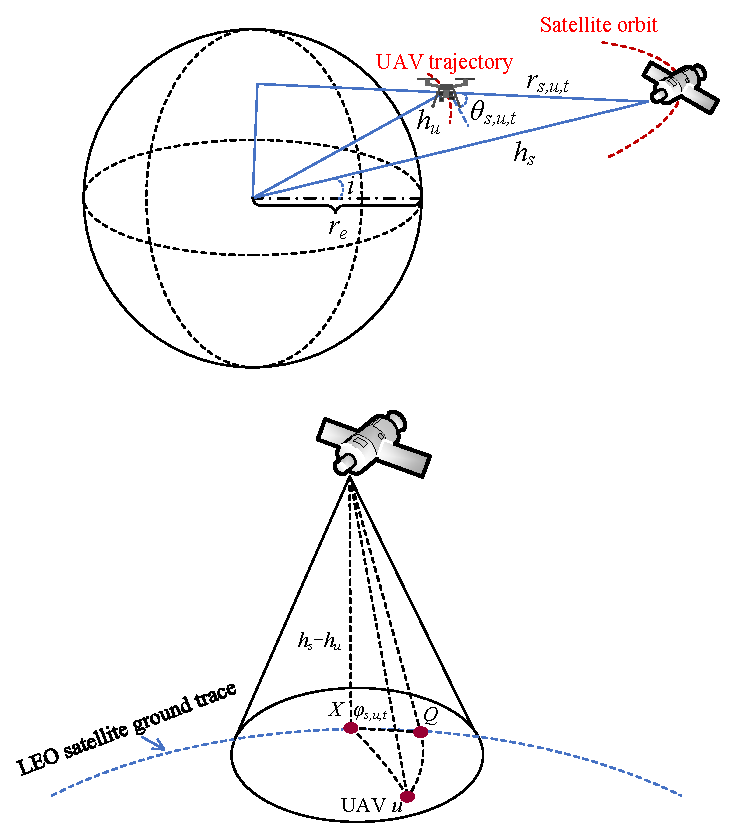
\includegraphics[width=0.95\columnwidth]{Definitions/figure2}
\caption{Geometric illustration of the UAV–LEO satellite link, including the satellite orbit, UAV position, Earth curvature, slant-range distance, and elevation angle, which together characterize the air-to-space propagation model employed in this study.}
\label{fig:uav_leo_geometry}
\end{figure}

A three-dimensional Cartesian coordinate system is adopted to describe the spatial distribution of UAVs and IoT devices. The IoT devices are randomly deployed on the ground plane, and the location of the $k$-th device is represented by $\mathbf{q}_k = (x_k, y_k, 0)$.
Each UAV maintains a constant altitude $h_u$; hence, its position at the $n$-th hovering point is given by $\mathbf{q}_u(n) = \big(x_u(n), y_u(n), h_u\big)$. 
Owing to the elevated UAV altitude and the predominantly unobstructed propagation conditions, the wireless links between IoT devices and UAVs are primarily characterized by line-of-sight (LoS) propagation. 
Accordingly, the channel gain between IoT device $k$ and its associated UAV is modeled as
\begin{equation}
d_k(n) = \sqrt{h_u^2 + (x_u(n) - x_k)^2 + (y_u(n) - y_k)^2},
\qquad
G_k = \frac{\beta_0}{d_k(n)^2}.
\end{equation}
where $\beta_0$ is the channel gain measured at the reference distance $r_0 = 1\,\text{m}$.

Let $\mathcal{P}$ denote the set of all feasible transmission pairs, where each pair $p \in \mathcal{P}$ consists of either (i) two IoT devices forming a NOMA cluster or (ii) a single device operating in OFDMA mode. 
A binary decision variable $\delta_{p} \in \{0,1\}$ is introduced to indicate whether pair $p$ is activated. 
To ensure that each IoT device participates in at most one transmission pair, the following constraint is imposed
\begin{equation}
    \sum_{p \in \mathcal{P}: k \in p} \delta_{p} \le 1, 
    \qquad \forall\, k \in \mathcal{K}.
\end{equation}

Given the pairing configuration, the received signal-to-interference-plus-noise ratio (SINR) of IoT device $k$ can be expressed as
\begin{equation}
\mathrm{SINR}_k 
= \frac{p_k G_k}{
    \displaystyle 
    \sum_{\substack{p \in \mathcal{P}: \, k\in p}} 
        \delta_p 
        \sum_{\substack{j \in p \\ j \neq k}} 
            p_j G_j 
    + \sigma_{iu}^2 },
\end{equation}
where $p_k$ is the transmit power of device $k$, and $\sigma_{iu}^2$ denotes the receiver noise power. 
The intra-pair interference term $\sum_{j \in p,\, j\neq k} p_j G_j$ appears only when the activated pair $p$ contains two devices. 
For NOMA pairs, the decoding order is determined by the channel gains, followingthe conventional successive interference cancellation (SIC) procedure.

Given the SINR expression, the achievable uplink data rate of device $k$ is 
\begin{equation}
d_k = B_{iu} \log_2\!\left(1 + \mathrm{SINR}_k\right),
\end{equation}
where $B_{iu}$ denotes the bandwidth allocated to UAV communications. 
For a task of size $D_k$, the corresponding uplink transmission delay is
\begin{equation}
T_k^{\mathrm{tr}} = \frac{D_k}{d_k}.
\end{equation}

After determining the trajectory of each UAV, a fixed visiting sequence is imposed to ensure that all NOMA clusters and singleton IoT devices are sequentially served. The trajectory of UAV~$u$ is denoted by the ordered set
\begin{equation}
\{\mathbf{q}_u(0), \mathbf{q}_u(1), \ldots, \mathbf{q}_u(N_u)\},
\end{equation}
where $N_u$ represents the number of hovering waypoints assigned to UAV~$u$. Accordingly, the total flight path length of UAV~$u$ throughout the mission is expressed as
\begin{equation}
L_u = \sum_{n=0}^{N_u-1} \left\| \mathbf{q}_u(n+1) - \mathbf{q}_u(n) \right\|_2,
\end{equation}
which captures the cumulative Euclidean distance traveled between consecutive hovering waypoints.

Given a constant flight speed $v_f$, the total flight time required by UAV~$u$ is calculated as
\begin{equation}
T_u^{\mathrm{fly}} = \frac{L_u}{v_f},
\end{equation}
where $L_u$ denotes the total flight path length of UAV~$u$. This expression follows directly from the definition of time as distance divided by speed under constant-velocity motion.

During the data collection phase, each UAV hovers at designated waypoints to receive data from the associated IoT devices. The hovering duration of UAV~$u$ depends on the transmission times of all active NOMA pairs and is given by
\begin{equation}
T_u^{\mathrm{hov}} = \sum_{p \in P} \delta_p \, \max_{k \in p} \frac{D_k}{d_k},
\end{equation}
where $\delta_p$ indicates whether pair $p$ is assigned to UAV~$u$, and the term $\max_{k \in p} \frac{D_k}{d_k}$ denotes the transmission time of pair~$p$, dominated by the device with the longest individual transmission time.

During this phase, the energy consumption of UAV~$u$ consists of both hovering energy and flight related energy. Accordingly, the total energy consumption is given by
\begin{equation}
E_{\text{total}} = \sum_{u=1}^{U} \left( P_h T_u^{\mathrm{hov}} + P_f T_u^{\mathrm{fly}} \right),
\end{equation}
where $P_h$ and $P_f$ denote the hovering power and flight power of the UAVs, respectively, and $T_u^{\mathrm{fly}}$ is the flight time of UAV~$u$ as defined earlier.

\subsection{Data Offloading from UAV to LEO}

After completing data collection from all IoT devices, each UAV obtains the position information of all visible LEO satellites and selects the satellite that can satisfy its offloading requirements.To represent the computation offloading decision, a binary association variable $\beta_{s,u,t} \in \{0,1\}$ is introduced, where $\beta_{s,u,t} = 1$ indicates that UAV~$u$ offloads its computation to satellite~$s$ at time slot~$t$. 

The large scale channel between UAV~$u$ and LEO satellite~$s$ is modeled using the free space path loss model, given in dB by
\begin{equation}
L^{\mathrm{fs}}_{s,u,t}(\mathrm{dB}) = 92.45 + 20\log_{10}(r_{s,u,t}) + 20\log_{10}(f_s),
\label{eq:fspl}
\end{equation}
where $f_s$ denotes the carrier frequency of satellite~$s$ in GHz. The line-of-sight distance $r_{s,u,t}$ is obtained from the geometric relationship illustrated in Fig.~\ref{fig:uav_leo_geometry}, given by
\begin{equation}
r_{s,u,t} = \sqrt{(r_e + h_s)^2 + (r_e + h_u)^2 - 2(r_e + h_s)(r_e + h_u) \cos \theta_{s,u,t}},
\end{equation}
where $r_e$ denotes the Earth radius, and $h_u$ and $h_s$ are the altitudes of the UAV and the LEO satellite, respectively.
 
The elevation angle $\theta_{s,u,t}$ between UAV~$u$ and satellite~$s$ is obtained from the satellite–UAV geometry shown in Fig.~\ref{fig:uav_leo_geometry} and is expressed as
\begin{equation}
\theta_{s,u,t} = \arctan \left( \frac{h_s - h_u}{d_{\mathrm{ground},s,u,t}} \right),
\label{eq:elevation} 
\qquad 
d_{\mathrm{ground},s,u,t} = r_e \phi_{s,u,t},
\end{equation}
where $d_{\mathrm{ground},s,u,t}$ denotes the ground-projected distance between UAV~$u$ and the sub-satellite point, and $\phi_{s,u,t}$ is the corresponding central angle on the Earth's surface. Following \cite{seyedi2012trace}, the central angle evolves over time as
\begin{equation}
\phi_{s,u,t} = (\omega_E \cos i - \omega_S)(t - t_0) + \phi_{s,u,t_0},
\end{equation}
where $\omega_E$ and $\omega_S$ denote the angular velocities of the Earth and satellite orbit, respectively, $i$ is the orbital inclination, $t_0$ is the time instant when the satellite becomes visible to the UAV, and $\phi_{s,u,t_0}$ is the initial central angle.

The received power at LEO satellite $s$ from UAV $u$ at time $t$ is given by
\begin{equation}
P_{s,u,t}^{\mathrm{re}} = P_{tr} G_{tr} G_{re} G_{s,u,t}^{\mathrm{lin}},
\end{equation}
where $P_{tr}$ denotes the UAV transmit power, $G_{tr}$ and $G_{re}$ are the transmit and receive antenna gains, and $G_{s,u,t}^{\mathrm{lin}}$ is the large-scale channel gain derived from the free-space path-loss model described in equation \eqref{eq:fspl}.

Based on the received power, the achievable uplink data rate from UAV $u$ to satellite~$s$ at time~$t$ follows the Shannon capacity expression
\begin{equation}
d_{s,u,t} = B_{su} \log_2\!\left(1 + \frac{P_{s,u,t}^{\mathrm{re}}}{\sigma_{su}^2} \right),
\label{eq:rate_equation}
\end{equation}
where $B_{su}$ is the allocated bandwidth of the UAV–LEO link and $\sigma_{su}^2 = N_0 B_{su}$ denotes the receiver noise power. Let $x_{s,u,t} \in \{0,1\}$ denote the satellite association decision, where $x_{s,u,t}=1$ indicates that UAV $u$ is connected to satellite $s$ at time $t$.

To account for unnecessary satellite switching, the handover indicator is defined as
\begin{equation}
h_{u,t} = \frac{1}{2} \sum_{s=1}^{S} \left| x_{s,u,t} - x_{s,u,t-1} \right|.
\end{equation}


\subsection{Problem Formulation}

To minimize the total energy consumption in the first-stage IoT--UAV data collection process, we jointly optimize the pair-selection variables $\boldsymbol{\delta}=\{\delta_p \mid p\in P\}$, the transmit-power allocation of IoT devices $\mathbf{p}=\{p_k \mid k\in K\}$, and the UAV hovering positions and visiting order $\mathbf{q}=\{\mathbf{q}_u(n) \mid u\in U\}$. The optimization problem is formulated as
\begin{subequations}
\begin{align}
\mathcal{P}_1: \
\min_{\boldsymbol{\delta},\mathbf{p},\mathbf{q}}
&\quad 
\sum_{u=1}^{U} \left( 
P_h \sum_{p \in P_u} \delta_p \max_{k\in p} \frac{D_k}{d_k}
+ P_f \frac{L_u}{v_f}
\right)
\label{eq:p1_obj} \\[4pt]
\text{s.t.}\quad
& p_{\min} \le p_k \le p_{\max}, && \forall k, 
\label{eq:p1_power} \\[2pt]
& \sum_{p: k\in p} \delta_p \le 1, && \forall k, 
\label{eq:p1_assignment} \\[2pt]
& \rho\, p_{i(p)} G_{i(p)} \le p_{j(p)} G_{j(p)}, && \forall p\in P_{\mathrm{NOMA}},
\label{eq:p1_noma} \\[2pt]
& \frac{p_k G_{k,u(p)}}{\sigma_u^2} \ge \gamma_{\min}, && \forall k \in p, \ \forall p \ \text{with } \delta_p=1,
\label{eq:p1_snr} \\[2pt]
& \|\mathbf{q}_u(n+1) - \mathbf{q}_u(n)\| \le v_{\max}\Delta t, && \forall u, \ \forall n,
\label{eq:p1_velocity} \\[2pt]
& \mathbf{q}_u(N_u) = \mathbf{q}_u(0), && \forall u,
\label{eq:p1_trajectory} \\[2pt]
& \delta_p \in \{0,1\}, && \forall p\in P.
\label{eq:p1_binary}
\end{align}
\end{subequations}

Constraint~\eqref{eq:p1_power} limits the transmit power of each IoT device to its feasible operating range.   
Constraint~\eqref{eq:p1_assignment} ensures that each device can participate in at most one NOMA pair.  
Constraint~\eqref{eq:p1_noma} guarantees the power-domain separation required for successful SIC decoding, where $i(p)$ and $j(p)$ denote the strong and weak users in pair $p$, respectively.  
Constraint~\eqref{eq:p1_snr} enforces the minimum SNR requirement needed for reliable uplink decoding at the UAV.  
Constraint~\eqref{eq:p1_velocity} ensures physically feasible UAV motion by restricting the maximum displacement between successive hovering points according to the UAV speed limit $v_{\max}$.  
Constraint~\eqref{eq:p1_trajectory} requires each UAV to complete a closed trajectory.  
Constraint~\eqref{eq:p1_binary} specifies the binary nature of the pairing decision variables.

Due to the intrinsic coupling among the discrete pairing variables, the continuous transmit-power variables, and the UAV trajectory variables, problem $\mathcal{P}_1$ is a mixed-integer nonlinear program (MINLP), which is generally NP-hard and computationally intractable to solve optimally.

After completing the IoT data-collection stage, each UAV proceeds to offload its aggregated task data to LEO satellites. The objective of the second-stage decision process is to minimize unnecessary handover events while guaranteeing the required offloading throughput. This improves QoS continuity and implicitly reduces both transmission and handover-related energy consumption.

The handover-aware satellite association problem is formulated as
\begin{subequations}
\begin{align}
\mathcal{P}_2: \ 
\min_{\mathbf{x}} \quad &
\sum_{u=1}^{U} \sum_{t=1}^{T} h_{u,t} \label{eq:p2_obj} \\[4pt]
\text{s.t.}\quad 
& \sum_{s=1}^{S} \sum_{t=1}^{T} x_{s,u,t} d_{s,u,t}\Delta t \ge D_u, 
&& \forall u,
\label{eq:p2_total}\\[2pt]
& \sum_{s=1}^{S} x_{s,u,t} \le 1, 
&& \forall u,\ \forall t,
\label{eq:p2_single}\\[2pt]
& x_{s,u,t} \le a_{s,u,t}, 
&& \forall s,u,t,
\label{eq:p2_elevation}\\[2pt]
& \sum_{s=1}^{S} \sum_{t'=t}^{T} x_{s,u,t'} d_{s,u,t'}\Delta t 
\ge D_u^{\mathrm{rem}}(t), 
&& \forall u,\ \forall t,
\label{eq:p2_remaining}\\[2pt]
& x_{s,u,t} \in \{0,1\}, 
&& \forall s,u,t. 
\label{eq:p2_binary}
\end{align}
\end{subequations}


Constraint~\eqref{eq:p2_total} ensures that the total successfully offloaded data meets the UAV's task requirement.  
Constraint~\eqref{eq:p2_single} restricts each UAV to associate with at most one satellite at each time slot.  
Constraint~\eqref{eq:p2_elevation} guarantees that association is allowed only when the satellite satisfies the minimum elevation angle,where $a_{s,u,t} \in \{0,1\}$ denotes the satellite visibility indicator,with $a_{s,u,t} = 1$ if $\theta_{s,u,t} \ge \theta_{\min}$ and $a_{s,u,t} = 0$ otherwise.  
Constraint~\eqref{eq:p2_remaining} avoids unnecessary switching by ensuring that the currently selected satellite can meet the remaining offloading demand under the predicted link evolution, where $D_u^{\mathrm{rem}}(t)$ denotes the remaining data to be uploaded at time~$t$.  
Constraint~\eqref{eq:p2_binary} specifies the binary nature of the association decisions.

Due to the temporal coupling of the binary association variables and the predicted throughput evolution, problem $\mathcal{P}_2$ is combinatorial and generally NP-hard. Thus, instead of computing the exact optimal solution, a demand-aware handover strategy is developed to obtain a practically efficient association policy.


\section{ALGORITHM DESIGN}

To efficiently solve the joint IoT–UAV data collection and UAV–LEO offloading problem, the proposed framework adopts a two-stage hierarchical design. In the first stage, corresponding to the IoT-to-UAV data transmission process, Algorithm~\ref{alg:p1_optimization} performs pair-based user grouping, transmit-power allocation, and UAV trajectory planning to minimize the UAV energy consumption. In the second stage, associated with the UAV-to-LEO offloading process, Algorithm~\ref{alg:satellite_selection} executes a demand-aware satellite selection strategy that mitigates unnecessary handovers while ensuring the required offloading throughput and QoS continuity.

\subsection{UAV Data Collection and Energy Optimization}

To effectively solve problem $\mathcal{P}_1$, we focus on minimizing the total UAV energy consumption incurred during the IoT–UAV data collection stage. Since the communication energy of IoT devices is negligible compared to the hovering and flight energy of UAVs, the optimization primarily targets the UAV energy components. The decision variables include the discrete pair-selection indicators $\boldsymbol{\delta}=\{\delta_p \mid p\in P\}$, the continuous transmit-power allocation $\mathbf{p}=\{p_k \mid k\in K\}$, and the UAV hovering positions $\mathbf{q}=\{\mathbf{q}_u(n)\mid u\in U\}$. 

The resulting problem is a MINLP characterized by tight coupling among discrete pairing decisions, continuous power variables, and geometric trajectory variables, making it computationally intractable to solve optimally. To address this challenge, we develop an alternating-optimization framework enhanced with a local-search refinement procedure. The overall algorithmic workflow is illustrated in Fig.~\ref{fig:algorithm_flowchart} and summarized in Algorithm~\ref{alg:p1_optimization}.

The initial NOMA pairs are formed using a distance-based greedy strategy. The pairwise distance matrix of all IoT devices is first computed, and the two closest devices that satisfy the NOMA feasibility constraints are grouped into a pair and added to the pair set $P$. This procedure is repeated until no additional valid pairs can be formed, and any remaining devices are treated as independent OFDMA users.

For each activated NOMA pair $p \in P$ with $\delta_p = 1$, an alternating-optimization procedure is executed to jointly refine the power allocation and UAV hovering position. Given a fixed UAV position $(x_u, y_u, h_u)$, the transmit powers of the paired devices are updated using a block coordinate descent (BCD) approach. Specifically, for each NOMA pair $p$, the transmit power of one user in $p$ is updated via a Newton-type step while the power of the other user is kept fixed, followed by a projection onto the feasible power domain to satisfy the NOMA decoding constraints. This process repeats until convergence. For OFDMA users, the transmit power is directly set to $p_{\max}$ to maximize the throughput and reduce hovering time.

With the power allocation fixed, the UAV hovering point $(x_u,y_u)$ ,where altitude $h_u$ kept constant, is refined using the Adam optimizer, which leverages momentum and adaptive learning rates to accelerate convergence compared with gradient-free heuristics. The update rule is
\begin{align}
\mathbf{m}_t &= \beta_1 \mathbf{m}_{t-1} + (1-\beta_1)\nabla_{\mathbf{q}} E_{\text{total}}, \\
\mathbf{v}_t &= \beta_2 \mathbf{v}_{t-1} + (1-\beta_2)(\nabla_{\mathbf{q}} E_{\text{total}})^2, \\
\mathbf{q}_u^{(t+1)} &= \mathbf{q}_u^{(t)} - \alpha \frac{\hat{\mathbf{m}}_t}{\sqrt{\hat{\mathbf{v}}_t} + \epsilon},
\end{align}
where $\mathbf{m}_t$ and $\mathbf{v}_t$ denote the first- and second-order moment estimates, and $\alpha$, $\beta_1$, and $\beta_2$ are the learning-rate and decay parameters, respectively. The alternating procedure iterates until reaching the maximum iteration count $J$ or until the reduction in objective value falls below a predefined threshold.

After determining all UAV hovering positions, the visiting order must be optimized to minimize the total flight distance. This routing subproblem is a variant of the multiple traveling salesman problem (mTSP). To refine the trajectory, the 2-opt local search algorithm is employed. In each iteration, two edges in the current tour are removed and reconnected in an alternative configuration. If the resulting trajectory shortens the total travel distance and eliminates path crossings, the update is accepted. The procedure is repeated until no further improvement is possible. Compared with metaheuristic approaches, 2-opt offers faster convergence and more stable performance for trajectory refinement in mTSP settings.

To further reduce energy consumption, a pair-recombination mechanism is introduced to enhance the NOMA pairing structure. Each unpaired device is examined to identify opportunities for forming a new NOMA pair with a member of an existing pair, provided that the resulting pair satisfies the NOMA decoding feasibility conditions. Similarly, for two spatially adjacent NOMA pairs, their members are evaluated for potential exchange if such a swap can reduce either UAV flight distance or hovering time while preserving NOMA constraints.

After each recombination or exchange operation, the UAV trajectory and the corresponding total energy consumption are recalculated. A new configuration is accepted only if it yields a strictly lower energy value; otherwise, the previous configuration is retained. By iteratively applying trajectory refinement and pairing-structure updates, the algorithm explores a broader solution space and achieves improved NOMA pairing and flight-path configurations. The full procedure is summarized in Algorithm~1, with the corresponding flowchart shown in Fig.~\ref{fig:algorithm_flowchart}.

\begin{figure*}[!t]
\centering
\resizebox{0.92\textwidth}{!}{%
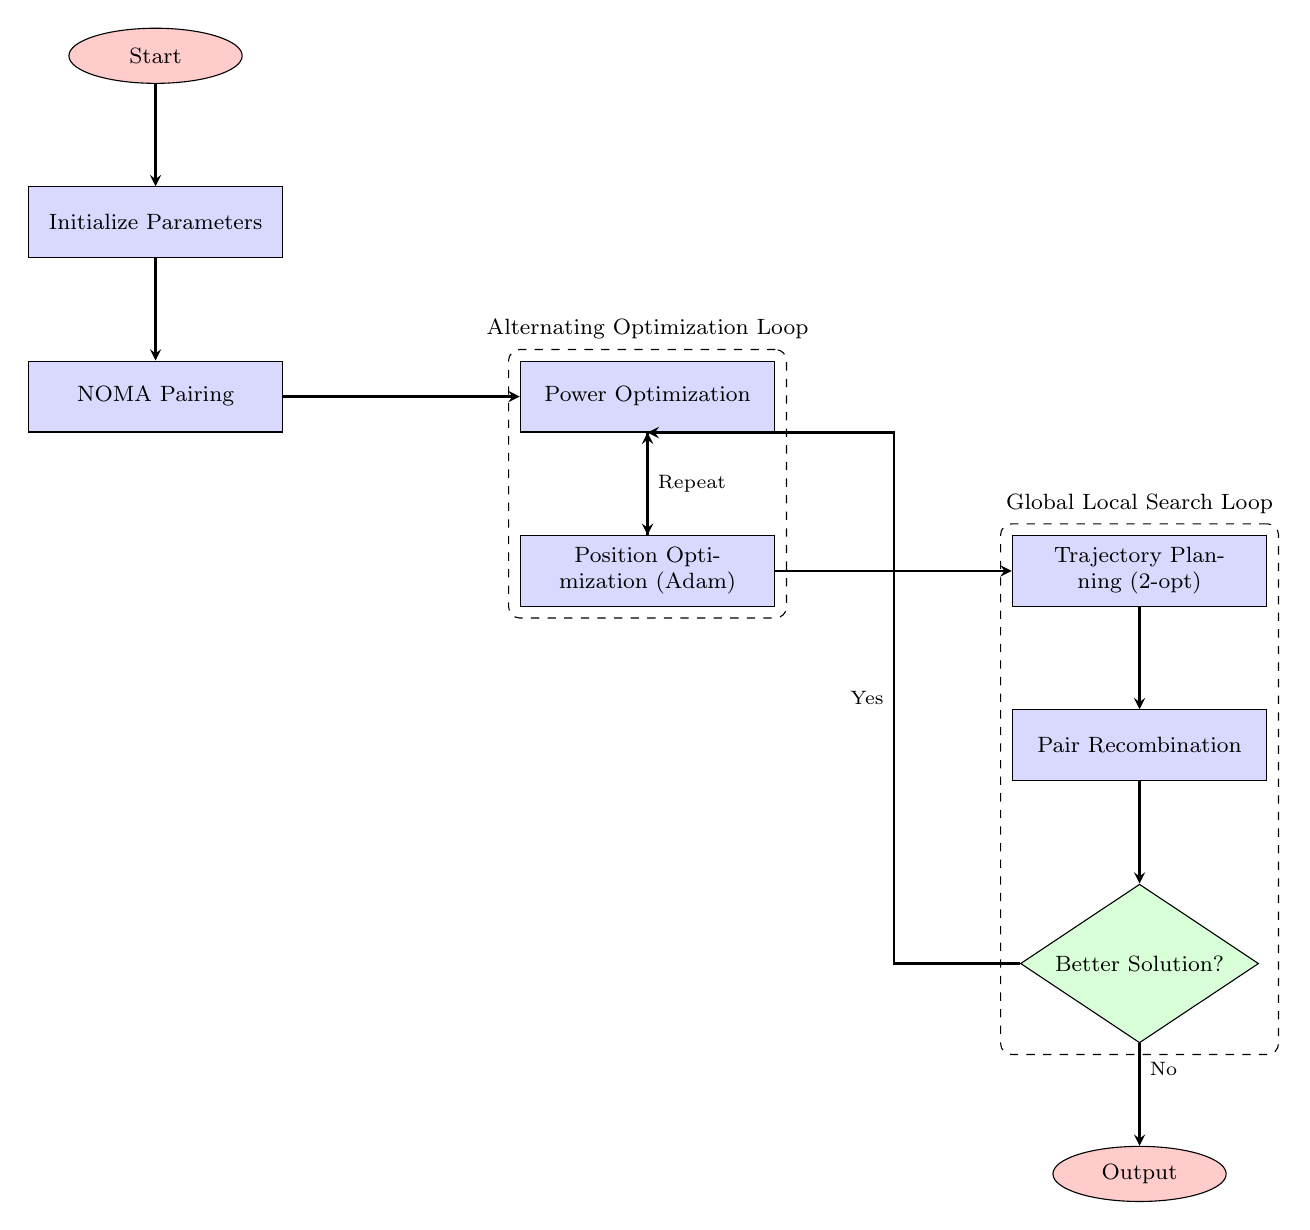
\begin{tikzpicture}[
    node distance=1.3cm and 2.4cm,
    startstop/.style={ellipse, draw, fill=red!20, text centered, minimum height=0.7cm, minimum width=2.2cm, font=\footnotesize},
    process/.style={rectangle, draw, fill=blue!15, text centered, text width=3cm, minimum height=0.9cm, font=\footnotesize},
    decision/.style={diamond, draw, fill=green!15, text centered, minimum height=1.2cm, minimum width=1.2cm, aspect=1.5, font=\footnotesize},
    dashedbox/.style={rectangle, draw, dashed, rounded corners, inner sep=4pt},
    arrow/.style={thick,->,>=stealth}
]

% ---------- 节点 ----------
% 第一列
\node (start) [startstop] {Start};
\node (init) [process, below=of start] {Initialize Parameters};
\node (pairing) [process, below=of init] {NOMA Pairing};

% 第二列:交替优化
\node (power) [process, right=3.0cm of pairing] {Power Optimization};
\node (position) [process, below=of power] {Position Optimization (Adam)};

% 第三列:全局局部搜索
\node (trajectory) [process, right=3.0cm of position] {Trajectory Planning (2-opt)};
\node (recombine) [process, below=of trajectory] {Pair Recombination};
\node (check) [decision, below=of recombine] {Better Solution?};
\node (stop) [startstop, below=of check] {Output};

% ---------- 主流程箭头 ----------
\draw [arrow] (start) -- (init);
\draw [arrow] (init) -- (pairing);
\draw [arrow] (pairing) -- (power);
\draw [arrow] (power) -- (position);

% 交替优化回环(完全在虚线框内)
\draw [arrow] (position.north) -- node[midway,right,font=\scriptsize] {Repeat} (power.south);

% 交替优化收敛后,进入轨迹规划
\draw [arrow] (position) -- (trajectory);

% 全局局部搜索部分
\draw [arrow] (trajectory) -- (recombine);
\draw [arrow] (recombine) -- (check);

% 决策结果箭头
\draw [arrow] (check) -- node[near start,right,font=\scriptsize] {No} (stop);
\draw [arrow] (check.west) -- ++(-1.6,0) |- 
      node[pos=0.25,left,font=\scriptsize] {Yes} (power.south);

% ---------- 虚线框 ----------
% 交替优化虚线框
\node[dashedbox, fit=(power) (position), label=above:{\footnotesize Alternating Optimization Loop}] (AObox) {};

% 全局局部搜索虚线框
\node[dashedbox, fit=(trajectory) (recombine) (check), label=above:{\footnotesize Global Local Search Loop}] (GSbox) {};

\end{tikzpicture}
}
\caption{Flowchart of the proposed UAV data collection algorithm with NOMA pairing, power control, and trajectory optimization.}
\label{fig:algorithm_flowchart}
\end{figure*}

\begin{algorithm}[!t]
\caption{UAV Data Collection and Energy Optimization}
\label{alg:p1_optimization}
\begin{algorithmic}[1]
    \State \textbf{Input:} IoT device locations $\{\mathbf{q}_k\}$, data sizes $\{D_k\}$, UAV initial position $\mathbf{q}_u(0)$
    \State \textbf{Output:} Total energy consumption $E_{\text{total}}$

    \Statex \Comment{Stage 1: Initial NOMA Pairing}
    \State Construct the distance matrix of all IoT devices
    \State Form the initial NOMA pair set $P$ using distance-based greedy pairing
    \State Let $U_{\text{solo}}$ be the set of unpaired devices

    \Statex \Comment{Stage 2: Alternating Optimization (Power $\leftrightarrow$ Position)}
    \State Initialize UAV hovering position $\mathbf{q}_u$
    \State Initialize transmit-power vector $\mathbf{p}$
    \For{$j = 1$ to $J$}
        \State Update $\mathbf{p}$ via Newton-type block coordinate descent with projection onto feasible power and NOMA constraints
        \State Update UAV hovering position $\mathbf{q}_u$ using the Adam optimizer
    \EndFor

    \Statex \Comment{Stage 3: Trajectory Optimization}
    \State Generate an initial visiting order for all UAV hovering waypoints
    \State Refine the trajectory using the 2-opt local search algorithm
    \State Compute the initial total energy $E_{\text{total}}$ using \eqref{eq:p1_obj}

    \Statex \Comment{Stage 4: Global Local Search with Pair Recombination}
    \Repeat
        \State $improved \gets \textbf{false}$
        \For{each NOMA pair $p \in P$}
            \For{each unpaired device $k \in U_{\text{solo}}$}
                \State Propose a recombination or user exchange between $k$ and pair $p$
                \If{the new pairing satisfies NOMA decoding constraints}
                    \State Re-run Stage~2 (power and position optimization)
                    \State Re-run Stage~3 (trajectory refinement)
                    \State Compute updated energy $E_{\text{new}}$
                    \If{$E_{\text{new}} < E_{\text{total}}$}
                        \State Accept the new configuration
                        \State $E_{\text{total}} \gets E_{\text{new}}$
                        \State $improved \gets \textbf{true}$
                    \Else
                        \State Reject the new configuration and revert to the previous one
                    \EndIf
                \EndIf
            \EndFor
        \EndFor
    \Until{$improved = \textbf{false}$}

    \State \Return $E_{\text{total}}$
\end{algorithmic}
\end{algorithm}


\subsection{LEO Satellite Selection Optimization}

After completing the data collection phase, the UAV must offload its aggregated information to LEO satellites for further processing. In contrast to stationary terrestrial ground stations, LEO satellites move rapidly along predetermined orbital trajectories, resulting in highly time-varying channel conditions and limited visibility windows. As a result, the satellite association decision plays a critical role in determining both the achievable uplink throughput and the stability of the communication link.
\begin{figure}[!t]
\centering
\resizebox{0.92\textwidth}{!}{%
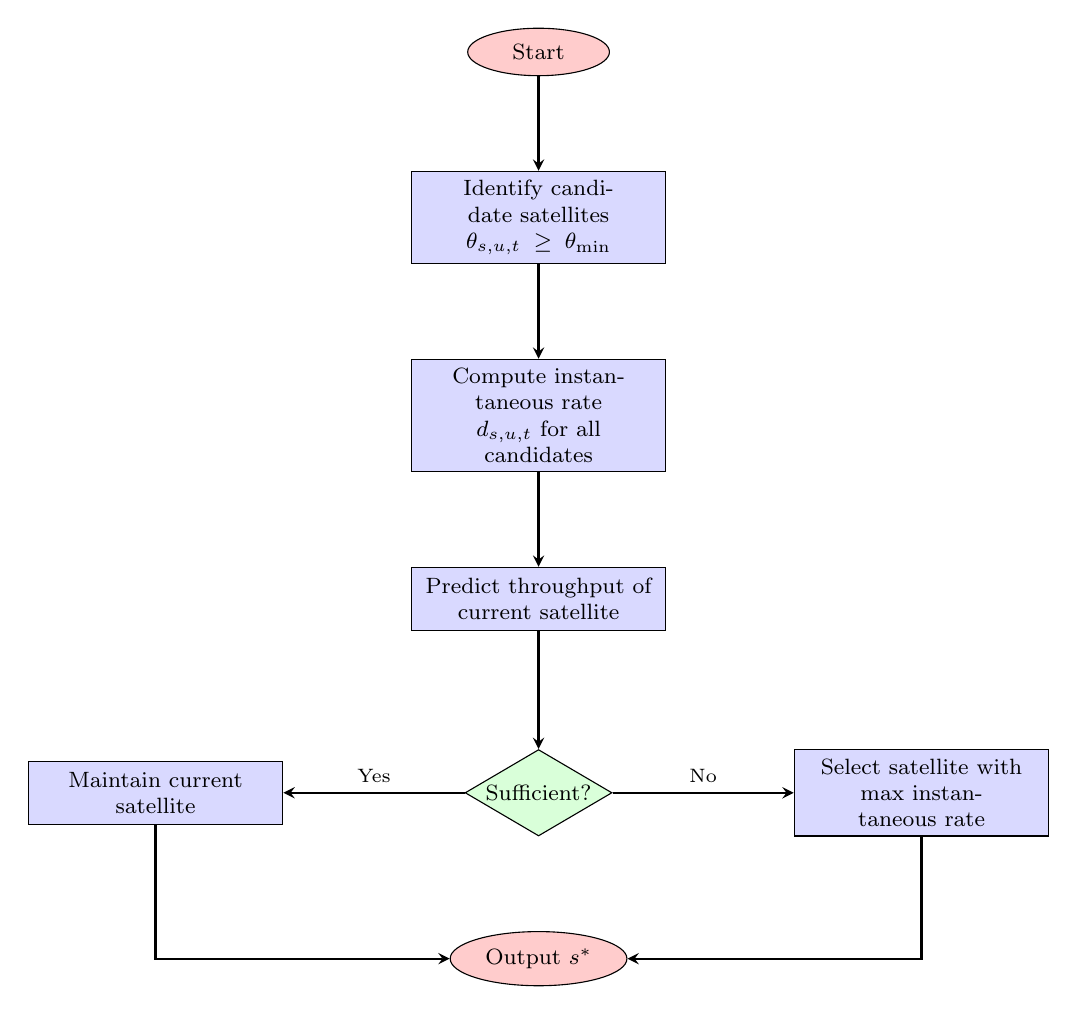
\begin{tikzpicture}[
    node distance=1.2cm and 2.2cm,
    startstop/.style={ellipse, draw, fill=red!20, text centered, minimum height=0.6cm, minimum width=1.8cm, font=\footnotesize},
    process/.style={rectangle, draw, fill=blue!15, text centered, text width=3cm, minimum height=0.8cm, font=\footnotesize},
    decision/.style={diamond, draw, fill=green!15, text centered, aspect=1.7, inner sep=1pt, font=\footnotesize},
    arrow/.style={thick,->,>=stealth}
]

% Nodes
\node (start) [startstop] {Start};
\node (cand) [process, below=of start] {Identify candidate satellites\\ $\theta_{s,u,t} \ge \theta_{\min}$};
\node (rate) [process, below=of cand] {Compute instantaneous rate\\ $d_{s,u,t}$ for all candidates};
\node (predict) [process, below=of rate] {Predict throughput of\\ current satellite};
\node (check) [decision, below=of predict, yshift=-0.3cm] {Sufficient?};
\node (keep) [process, left=2.3cm of check] {Maintain current\\ satellite};
\node (switch) [process, right=2.3cm of check] {Select satellite with\\ max instantaneous rate};
\node (stop) [startstop, below=1.2cm of check] {Output $s^*$};

% Arrows
\draw [arrow] (start) -- (cand);
\draw [arrow] (cand) -- (rate);
\draw [arrow] (rate) -- (predict);
\draw [arrow] (predict) -- (check);

\draw [arrow] (check) -- node[above, font=\scriptsize]{Yes} (keep);
\draw [arrow] (check) -- node[above, font=\scriptsize]{No} (switch);

\draw [arrow] (keep) |- (stop);
\draw [arrow] (switch) |- (stop);

\end{tikzpicture}
}
\caption{Flowchart of the demand-aware LEO satellite selection algorithm.}
\label{fig:leo_selection_flowchart}
\end{figure}

Frequent satellite handovers lead to increased signaling overhead, potential packet loss, and service interruptions, thereby degrading the overall quality of service. On the other hand, maintaining a connection to a satellite with deteriorating link quality prolongs transmission time and increases energy consumption. Hence, an effective association strategy must carefully balance the tradeoff between reducing unnecessary handovers and preserving sufficient link quality to ensure timely and reliable data offloading.

To address problem $\mathcal{P}_2$, a demand-aware satellite selection mechanism is proposed. Instead of adopting a greedy policy that always associates with the satellite providing the highest instantaneous throughput, the proposed algorithm assesses whether the currently connected satellite can still satisfy the remaining offloading demand based on the predicted link evolution. A handover is triggered only when the projected achievable throughput of the current link becomes insufficient to complete the remaining task, thereby avoiding unnecessary switching while ensuring timely and reliable data delivery.

At each decision epoch, all LEO satellites satisfying the elevation constraint $\theta_{s,u,t} \ge \theta_{\min}$ are identified as candidate satellites. For each candidate $s$, the instantaneous uplink rate $d_{s,u,t}$ is computed using \eqref{eq:rate_equation} based on the distance-dependent channel gain. The algorithm then predicts the cumulative throughput that the currently associated satellite can provide over its remaining visibility window. If this predicted throughput exceeds the remaining data requirement $D_u^{\mathrm{rem}}(t)$, the current association is maintained. Otherwise, a handover is initiated to the candidate satellite offering the maximum instantaneous throughput.

\begin{algorithm}[!t]
\caption{Demand-Aware LEO Satellite Selection}
\label{alg:satellite_selection}
\begin{algorithmic}[1]

\State \textbf{Input:} UAV position $\mathbf{q}_u(t)$, total data size $D_u$, transmitted data $D_u^{\text{tx}}$, current satellite $s_{\text{curr}}$, current time $t$
\State \textbf{Output:} Selected satellite $s^*$

\State Compute remaining data $D_u^{\text{rem}}(t) \gets D_u - D_u^{\text{tx}}$

\State Initialize candidate set $\mathcal{S}_{\text{cand}} \gets \emptyset$

\For{each satellite $s \in \mathcal{S}$}
    \State Compute elevation angle $\theta_{s,u,t}$ using \eqref{eq:elevation}
    \If{$\theta_{s,u,t} \ge \theta_{\min}$}
        \State $\mathcal{S}_{\text{cand}} \gets \mathcal{S}_{\text{cand}} \cup \{s\}$
    \EndIf
\EndFor

\If{$s_{\text{curr}} \in \mathcal{S}_{\text{cand}}$}
    \State Predict visibility window end time $t_{\text{exit}}(s_{\text{curr}})$
    \State $T_{\text{vis}} \gets t_{\text{exit}}(s_{\text{curr}}) - t$
    \State Predict future achievable throughput:
    \[
        \hat{D}_{\text{curr}} \gets \sum_{t'=t}^{t_{\text{exit}}} d_{s_{\text{curr}},u,t'} \Delta t
    \]
    \If{$\hat{D}_{\text{curr}} \ge D_u^{\text{rem}}(t)$}
        \State \Return $s_{\text{curr}}$ \Comment{Current link sufficient, no handover}
    \EndIf
\EndIf

\State Choose the best candidate:
\[
    s^* \gets \arg\max_{s \in \mathcal{S}_{\text{cand}}} d_{s,u,t}
\]
\State \Return $s^*$

\end{algorithmic}
\end{algorithm}


%%%%%%%%%%%%%%%%%%%%%%%%%%%%%%%%%%%%%%%%%%
\section{SIMULATION RESULTS}

The performance of the proposed two-stage optimization framework is evaluated through extensive simulations. The evaluation covers both individual stages—UAV-assisted IoT data collection and LEO satellite offloading—as well as their end-to-end integration. All numerical parameters are summarized in Table~\ref{tab:sim_parameters}, and the experiments are implemented in Python~3.10 on a workstation equipped with an Intel Core i7-12700K CPU and 32~GB RAM.
\begin{table}[!htbp]
\centering
\caption{Simulation Parameters}
\label{tab:simulation_parameters}
\begin{tabular}{llll}
\toprule
\textbf{Parameter} & \textbf{Value} & \textbf{Parameter} & \textbf{Value} \\
\midrule
$K$ (IoT devices) & 20 & $N$ (hover points) & 10 \\
$D_k$ (data size) & 10 MB & $B_{iu}$ & 1 MHz \\
$P_{\max}$ & 5 W & $P_{\min}$ & 0.1 W \\
$P_h$ & 100 W & $P_f$ & 150 W \\
$v_f$ & 10 m/s & $h_u$ & 100 m \\
$\beta_0$ & $10^{-5}$ & $\sigma^2_{iu}$ & $10^{-9}$ W \\
$\rho$ & 0.8 & $d_{\max}$ & 100 m \\
Area size & $500 \times 500$ m$^2$ & $\alpha$ (Adam) & 0.01 \\
$\beta_1$ (Adam) & 0.9 & $\beta_2$ (Adam) & 0.999 \\
$J$ (max iterations) & 100 & $\epsilon$ & $10^{-6}$ \\
\bottomrule
\end{tabular}
\end{table}

\begin{table}[!htbp]
\centering
\caption{LEO Satellite Parameters}
\label{tab:leo_parameters}
\begin{tabular}{llll}
\toprule
\textbf{Parameter} & \textbf{Value} & \textbf{Parameter} & \textbf{Value} \\
\midrule
$\theta_{\min}$ & 15$^\circ$ & $B_{su}$ & 10 MHz \\
$P_{tr}$ & 10 W & $G_{tr}$ & 10 dBi \\
$G_{re}$ & 30 dBi & $\sigma^2_{su}$ & $4 \times 10^{-14}$ W \\
$f_s$ & 20 GHz & $r_e$ & 6378 km \\
$h_s$ (LEO altitude) & 550 km & $\omega_E$ & 7.29 rad/s \\
Constellation & Starlink & Num. satellites & 200 \\
\bottomrule
\end{tabular}
\end{table}
% Figure 4
\begin{figure}[!htbp]
\centering
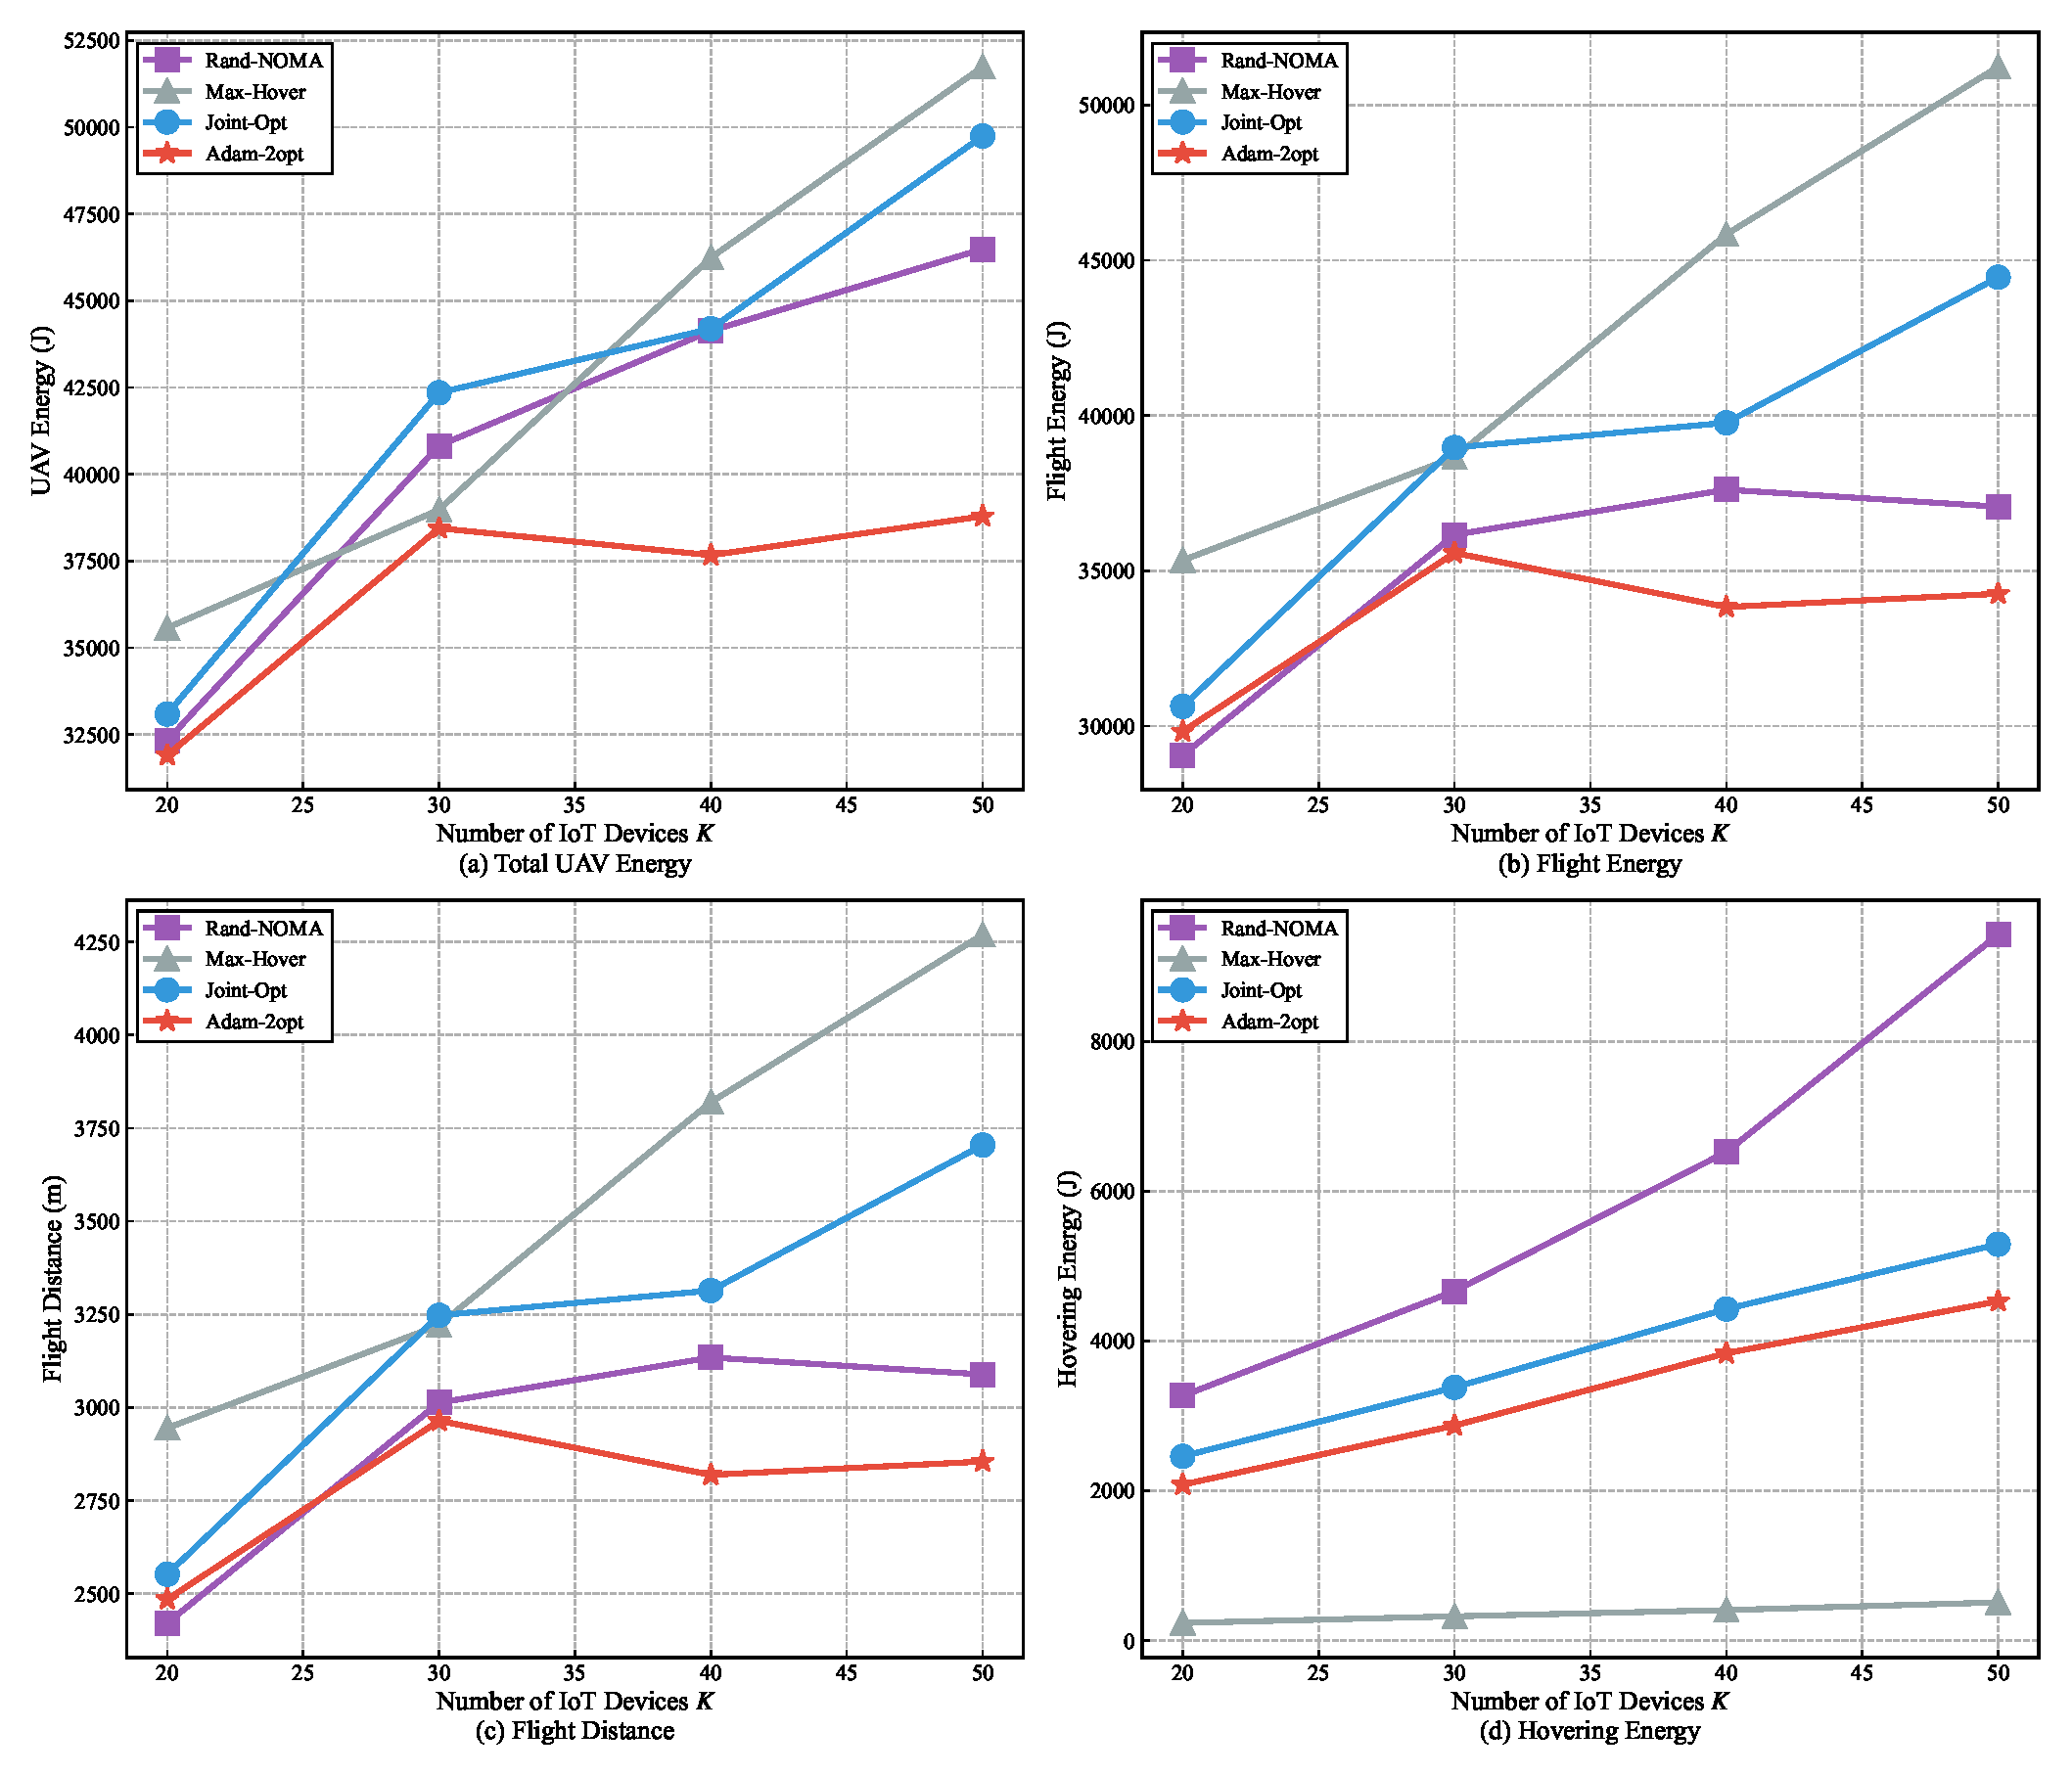
\includegraphics[width=0.95\columnwidth]{Definitions/comparison_4algorithms}
\caption{Performance comparison of different algorithms in the IoT-UAV phase.}
\label{fig:comparison_4algorithms}
\end{figure}
The first part of the evaluation focuses on the ground-to-air segment. UAVs operate within a $500\times 500~\text{m}^2$ area containing spatially distributed IoT devices, and a fixed-altitude multi-UAV configuration is adopted to reflect typical low-altitude urban deployments. Each scenario is executed under three independent random seeds, and results are averaged. To assess the effectiveness of the proposed Adam-2opt algorithm, three baseline strategies are considered: (i) \textit{Random Pairing}, which forms NOMA pairs without channel awareness; (ii) \textit{Fixed Hovering}, which prioritizes hovering duration without optimizing flight paths; and (iii) \textit{Basic Optimization}, which incorporates pairing, power allocation, and position optimization but lacks trajectory refinement.
% Figure 5
\begin{figure}[!htbp]
\centering
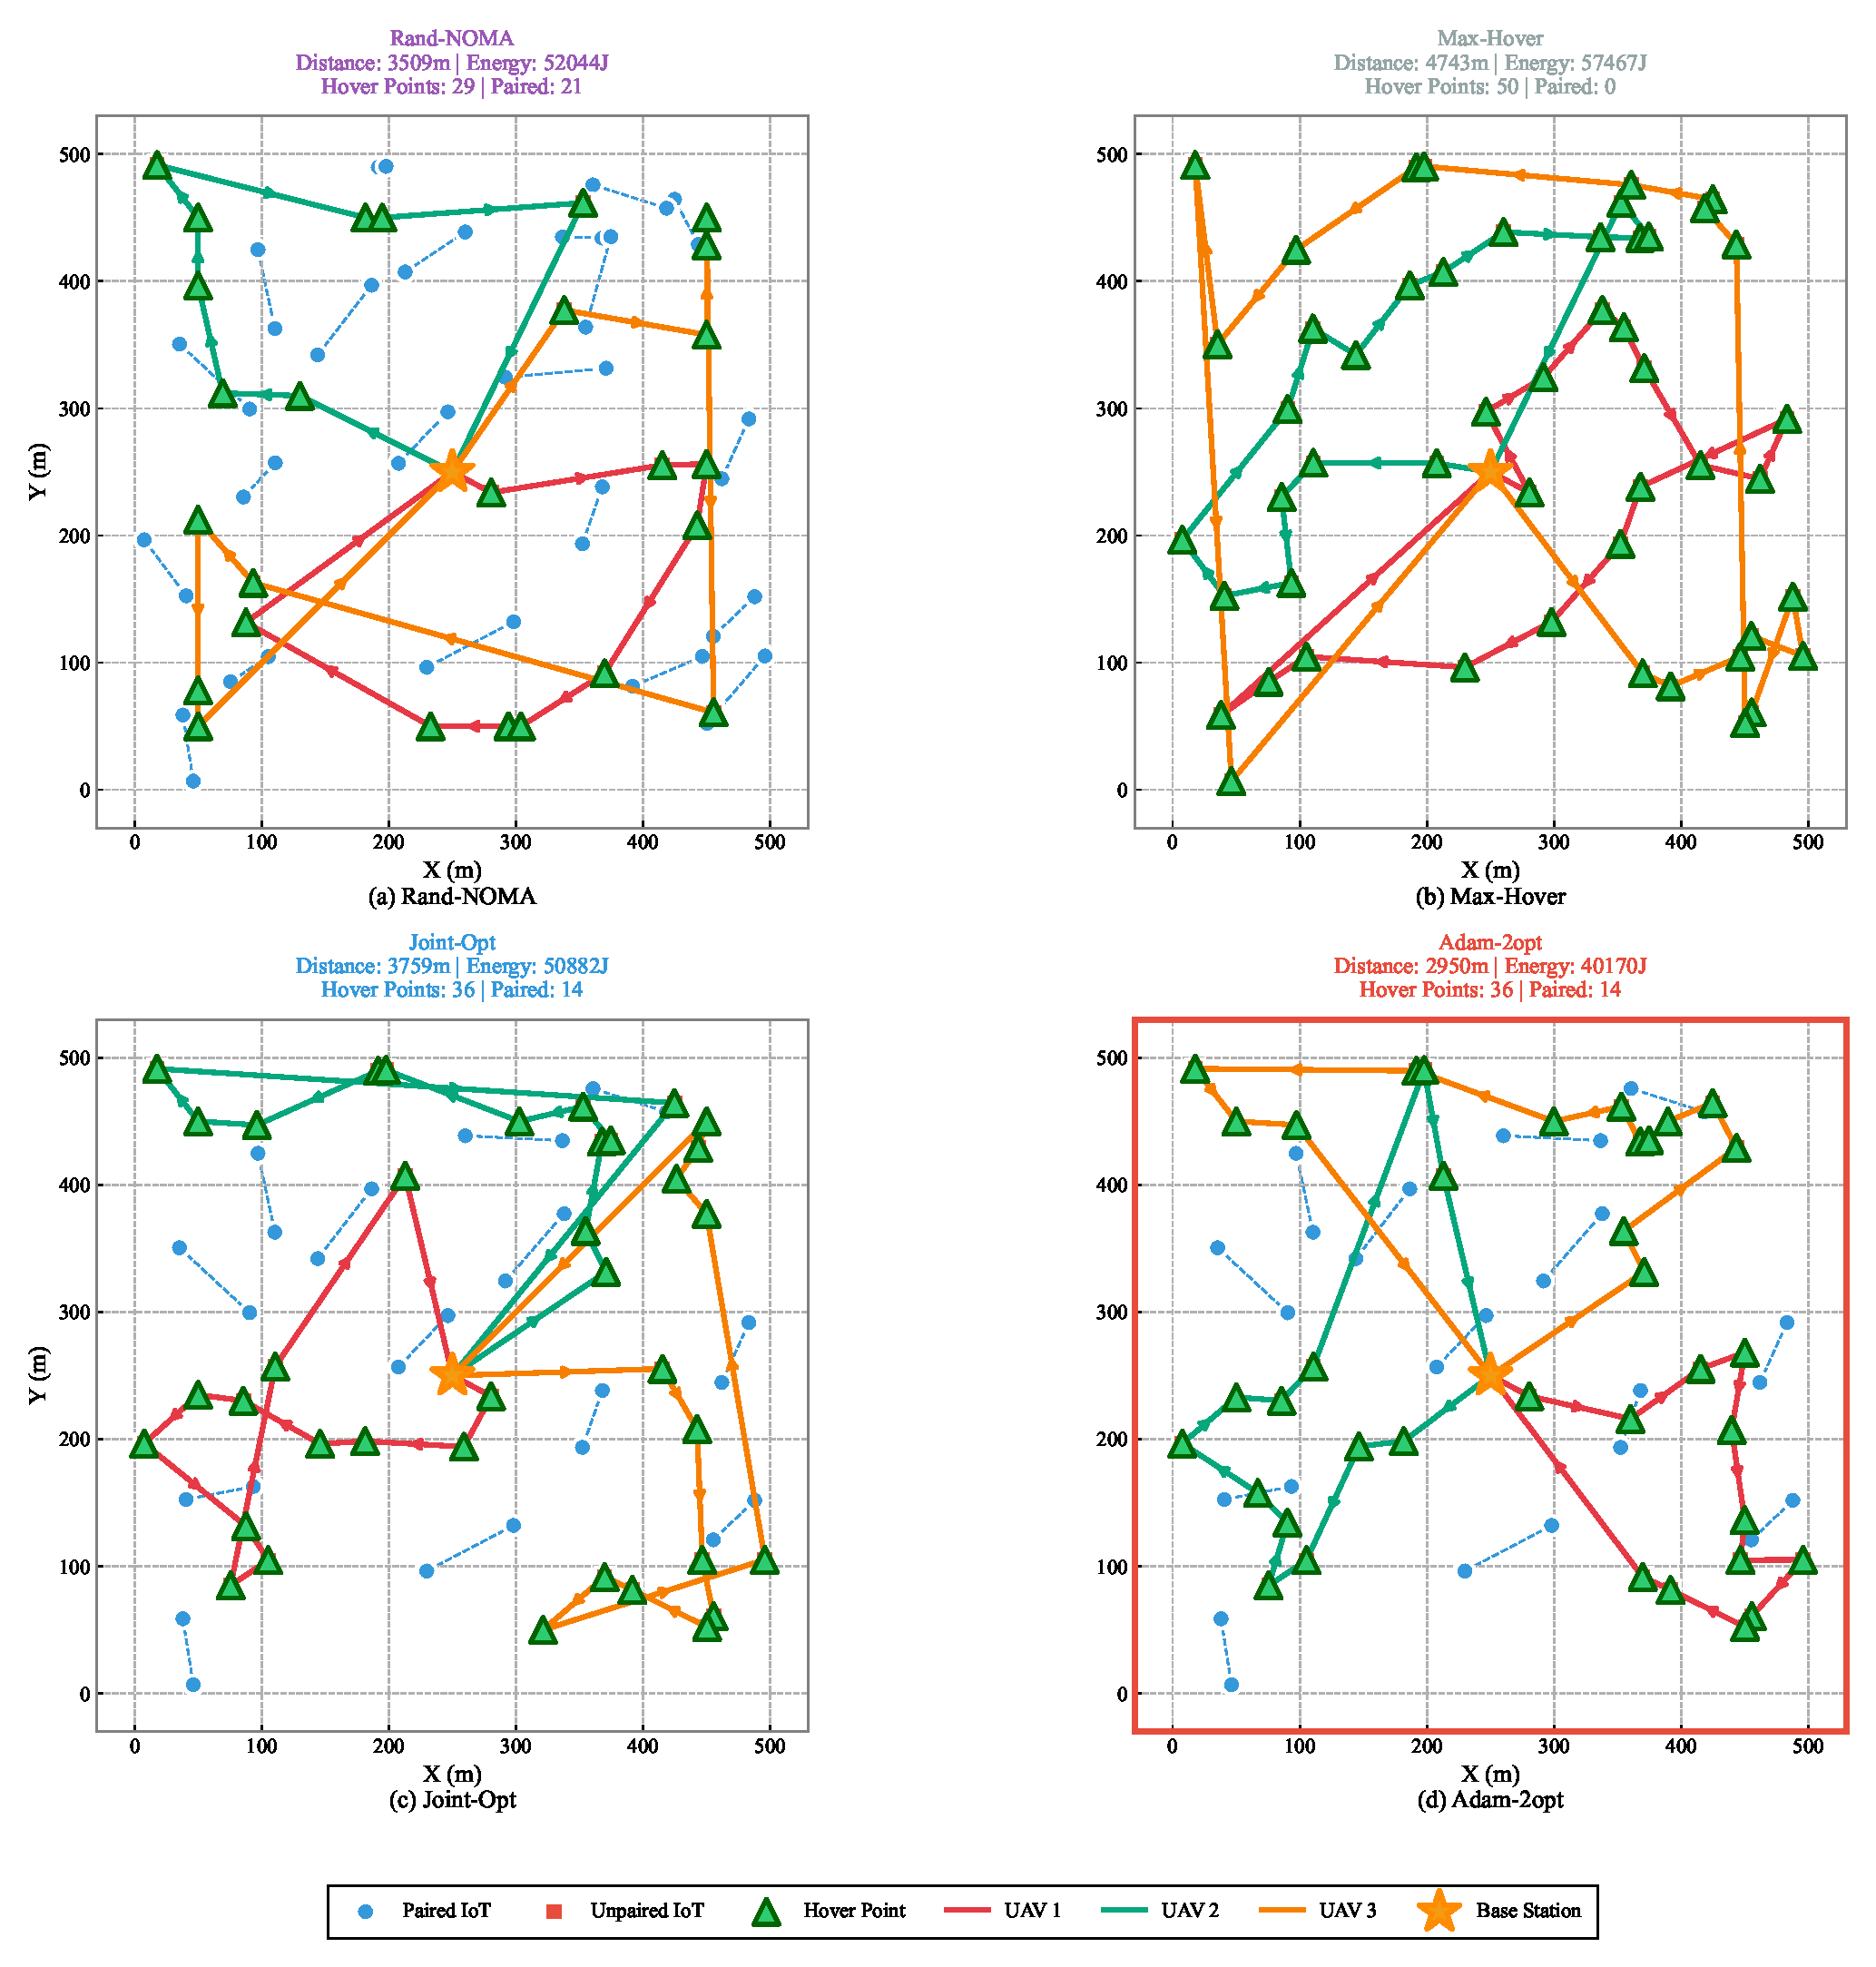
\includegraphics[width=0.95\columnwidth]{Definitions/trajectory_comparison_4algorithms}
\caption{UAV trajectory comparison between different optimization algorithms.}
\label{fig:trajectory_comparison}
\end{figure}
The second part of the evaluation examines the air-to-space offloading process. The Starlink constellation at 550~km altitude is simulated, and the number of visible satellites varies with time as the orbital geometry evolves. The UAV employs a 20~GHz carrier frequency and adheres to a minimum elevation angle constraint. A fixed interruption duration is applied to each handover event. A 10-minute evaluation window with 20-second intervals is considered, during which multiple handover opportunities arise. Two handover strategies are compared: a \textit{Greedy} scheme that always selects the satellite offering the highest instantaneous rate, and the proposed \textit{Demand-Aware} method, which performs handover only when necessary to meet the remaining offloading demand.


\subsection{Ground-to-Air Data Acquisition Performance}

The ground-to-air data acquisition stage poses a tightly coupled optimization problem involving NOMA pairing, power allocation, and UAV trajectory design. Figure~\ref{fig:comparison_4algorithms} summarizes the performance of all evaluated algorithms across four key metrics. The results consistently show that the proposed Adam-2opt method delivers the most energy-efficient operation, particularly in dense IoT deployments.

Figure~\ref{fig:comparison_4algorithms}a indicates that total UAV energy consumption increases with the number of IoT devices, yet the proposed method exhibits the slowest growth trend. While all algorithms perform similarly under low-density conditions ($K=20$), the performance gap widens significantly as the network scales. At $K=50$, Adam-2opt achieves more than 16\% energy reduction compared with Random Pairing, and over 22\% compared with Basic Optimization. This demonstrates that advanced trajectory refinement becomes increasingly valuable when device clustering and route complexity intensify. 

The primary advantage of Adam-2opt arises from its ability to simultaneously optimize hovering locations and visit sequencing. As shown in Figure~\ref{fig:comparison_4algorithms}c, the proposed design produces the shortest flight distance among all methods, with a reduction exceeding 30\% relative to Fixed Hovering at high densities. The 2-opt refinement eliminates path crossings and unnecessary detours, which directly translates into reduced flight energy, as reflected in Figure~\ref{fig:comparison_4algorithms}b. These improvements highlight the importance of trajectory-level optimization in UAV-assisted data collection.

Hovering energy behavior, depicted in Figure~\ref{fig:comparison_4algorithms}d, provides additional insight into algorithmic trade-offs. Fixed Hovering minimizes hovering time by construction but suffers from excessive flight distance, leading to the highest overall energy consumption. Random Pairing exhibits the opposite issue: arbitrary device grouping produces spatially dispersed clusters, substantially increasing hovering duration. By contrast, Adam-2opt maintains balanced performance—hovering time is reduced by nearly 50\% compared with Random Pairing—while preserving the shortest flight trajectory. This balanced design is essential for missions where both hovering and flight energy dominate total consumption.

To further illustrate spatial efficiency, Figure~\ref{fig:trajectory_comparison} visualizes representative flight paths for $K=50$. The Random Pairing trajectory (Figure~\ref{fig:trajectory_comparison}a) displays numerous crossings and backtracking segments, consistent with the disordered pairing structure. Fixed Hovering (Figure~\ref{fig:trajectory_comparison}b) generates well-spread hovering points but forces UAVs to traverse a large number of redundant waypoints. Basic Optimization (Figure~\ref{fig:trajectory_comparison}c) improves spatial locality but still retains avoidable turns and suboptimal visiting sequences. The proposed Adam-2opt trajectory (Figure~\ref{fig:trajectory_comparison}d) is notably more compact and structured, with no crossings and a clear directional flow. This confirms the complementary roles of Adam-based hovering refinement and 2-opt sequencing in producing globally efficient flight paths.

Computational cost results show that Adam-2opt requires greater planning time due to its iterative nature. However, the runtime remains on the order of one second, which is negligible for offline mission planning. The energy savings achieved—exceeding 16\% in dense deployments—far outweigh this cost, reinforcing the practicality of the approach for pre-scheduled UAV operations.

Finally, the scalability trends observed in Figure~\ref{fig:comparison_4algorithms} underline an important system-level implication. While simple heuristics suffice in small networks, their performance deteriorates rapidly with increasing density. In contrast, Adam-2opt exhibits sublinear growth in energy consumption and maintains robust performance as $K$ increases. This indicates that the proposed framework is particularly well-suited for large-scale IoT scenarios where spatial clustering and route complexity demand more sophisticated optimization.


% ==============================================================================
% 4.3 Performance of UAV-LEO Offloading Stage
% ==============================================================================
\subsection{UAV–LEO Offloading Performance}

The second stage evaluates the offloading of aggregated data from UAVs to LEO satellites, where the dominant challenge shifts from spatial optimization to managing strongly time-varying satellite visibility. Unlike the ground-to-air segment, satellite links exhibit rapid fluctuations due to orbital motion, making connection stability as critical as instantaneous link quality.
% Figure 6
\begin{figure}[!htbp]
\centering
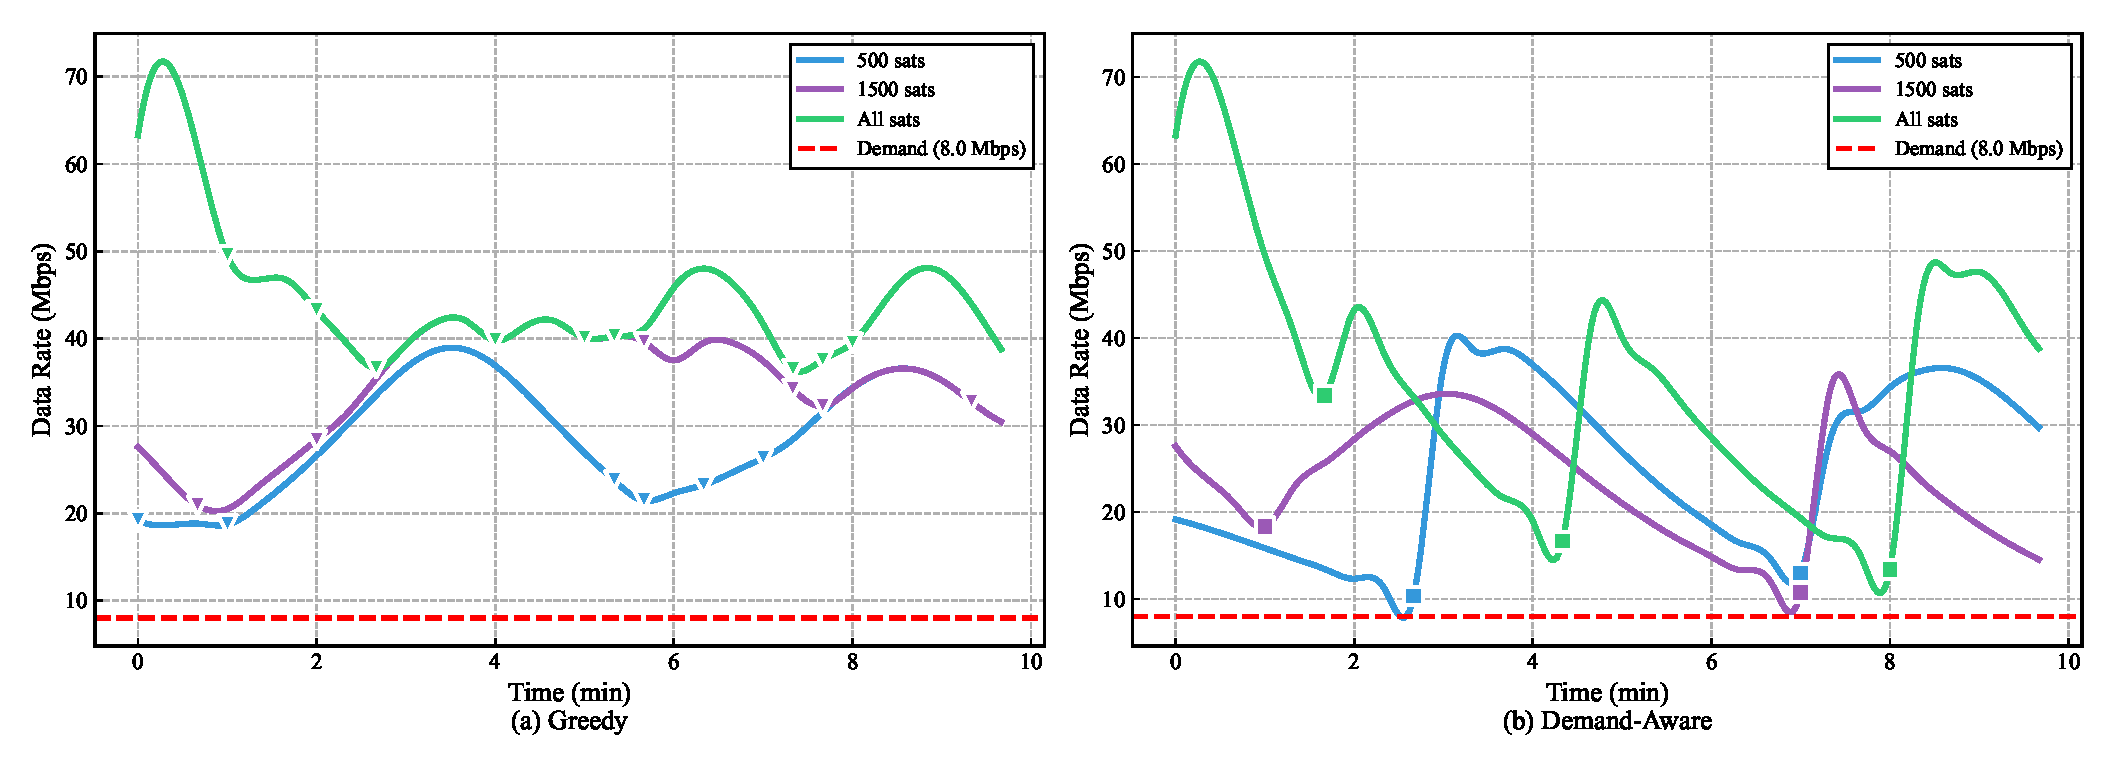
\includegraphics[width=0.95\columnwidth]{Definitions/demand_aware_number_of_satellites}
\caption{Comparison of satellite selection strategies: handover frequency versus constellation size.}
\label{fig:demand_aware_satellites}
\end{figure}
A key observation from Figure~\ref{fig:demand_aware_satellites} is the fundamental difference in handover behavior between the two evaluated strategies. The Greedy scheme continually switches to the satellite offering the highest instantaneous rate, resulting in pronounced rate volatility and frequent handover events. This behavior becomes more severe as satellite density increases, reflecting its sensitivity to instantaneous channel variations rather than long-term transmission feasibility.

In contrast, the Demand-Aware strategy produces consistently smoother rate trajectories and dramatically fewer handovers. By maintaining the current satellite connection as long as the remaining data demand can be satisfied within the predicted visibility window, the method avoids unnecessary switching and preserves link continuity. This design principle leads to a stable operating regime across all constellation densities, with only two to three handovers observed even in large constellations.
% Figure 6
\begin{figure}[!htbp]
\centering
\includegraphics[width=0.95\columnwidth]{Definitions/packet_loss_analysis}
\caption{Impact of satellite selection strategy on packet loss performance.}
\label{fig:packet_loss}
\end{figure}
Figure~\ref{fig:packet_loss}a quantitatively highlights this stability. Demand-Aware consistently reduces handover occurrences by 66--75\% relative to Greedy, and the reduction remains nearly invariant across the 500-, 1500-, and full-constellation scenarios. This invariance is particularly notable because it shows that the strategy scales gracefully with constellation size: the number of available satellites increases, but the handover count does not. Thus, Demand-Aware does not exploit satellite density to switch more frequently; instead, it leverages it to sustain longer, more reliable connections.

The practical implication of reduced handover activity is evident in the packet loss performance shown in Figure~\ref{fig:packet_loss}b. Because every handover incurs a fixed interruption period, lower switching frequency directly translates into proportionally lower loss rates. Demand-Aware maintains packet loss between 0.133\% and 0.200\%, whereas Greedy experiences losses three to four times higher. Although the absolute percentages appear small, the difference corresponds to several tens of kilobits over a typical mission—non-negligible for latency-sensitive applications such as real-time sensing or video uplink. These results demonstrate that optimizing for stability can yield a more reliable offloading process than purely maximizing instantaneous rate.

A trade-off emerges when examining average throughput. The Greedy strategy attains higher mean rates due to its aggressive switching behavior; however, this throughput advantage comes at the cost of substantial instability, packet loss, and service disruption. Demand-Aware yields 13--32\% lower average rates, but still consistently exceeds the required 8~Mbps demand by a comfortable margin. This surplus indicates that the system is operating well above its QoS threshold even without chasing maximum instantaneous rate, validating that rate maximization is not the limiting factor in this stage.

Finally, the scalability behavior across constellations provides insight into future LEO deployments. As the density of satellites increases, Greedy becomes increasingly unstable, with handover counts rising due to more frequent rate fluctuations. Demand-Aware, however, maintains nearly identical performance across all densities. This robustness arises from its demand-driven decision rule, which depends on the time required to complete the remaining offloading task rather than on short-term channel variations. Consequently, the method remains effective even as constellation sizes grow, making it well-suited for next-generation, high-density LEO systems.


\subsection{End-to-End System Analysis}

The end-to-end evaluation highlights how the two-stage optimization framework jointly enhances mission efficiency from initial IoT data acquisition to final satellite offloading. While the preceding subsections examined each stage independently, their combined behavior reveals the full benefit of coupling spatial efficiency in the ground segment with temporal stability in the space segment.

A representative mission with $K=50$ devices and 500 visible satellites illustrates this interaction. In the acquisition stage, the Adam-2opt method completes data collection with substantially reduced flight distance and energy expenditure, resulting in a shorter collection period. This improvement has direct implications for the offloading stage: by shortening the time window during which data must be transmitted, and by generating well-structured aggregated traffic, the system lowers the temporal pressure placed on the satellite link.

The offloading stage further amplifies these gains. The Demand-Aware strategy maintains stable connectivity with only two satellite handovers while sustaining data rates well above the required threshold. The reduced switching activity not only minimizes packet loss but also prevents retransmissions that would otherwise increase mission duration and UAV energy consumption. Together, the two stages form a complementary pair: the first minimizes the amount of work the second must perform under dynamic link conditions, while the second ensures reliable and efficient transfer of the data produced by the first.

Table~\ref{tab:end_to_end_comparison} summarizes the resulting system-level improvements. The proposed framework achieves simultaneous reductions in UAV energy consumption, flight distance, collection time, handover count, and packet loss. Although the average offloading rate is modestly lower than that of the Greedy strategy, it remains well above the demand threshold, confirming that meeting quality-of-service requirements does not require maximizing instantaneous throughput. Instead, the results show that stability-driven offloading yields superior system performance across all metrics of operational relevance.

The scalability characteristics further emphasize the robustness of the design. As IoT device density increases, the benefits of spatial optimization become more pronounced, with energy savings rising from marginal levels at low density to double-digit improvements at higher density. Conversely, the performance of the offloading stage remains largely unaffected by ground-segment scaling, consistently limiting handovers to two or three events regardless of IoT density. This decoupling is desirable: Algorithm~1 efficiently adapts to spatial complexity on the ground, while Algorithm~2 maintains stable performance in the space segment independent of the ground network.

Satellite density variation produces a similar conclusion. The Greedy strategy becomes increasingly unstable as constellation density grows, whereas the Demand-Aware approach exhibits nearly constant switching behavior. This insensitivity to satellite availability reflects a fundamental advantage of demand-based switching: decisions are driven by transmission requirements rather than by short-term channel fluctuations. As next-generation LEO constellations continue to expand, such robustness will be essential for ensuring reliable large-scale UAV–satellite integration.

Overall, the end-to-end evaluations demonstrate that optimizing spatial and temporal dimensions jointly, rather than individually, yields substantial system-level gains. By aligning the objectives of ground-level trajectory design with those of satellite-level handover management, the proposed framework supports efficient, reliable, and scalable operation across heterogeneous segments of the SAGIN architecture.

%%%%%%%%%%%%%%%%%%%%%%%%%%%%%%%%%%%%%%%%%%
\section{Discussion}

The simulation results provide several overarching insights into the design of integrated UAV-assisted IoT collection and LEO satellite offloading systems. Beyond validating the performance gains of the proposed algorithms, the findings highlight structural principles that can inform future SAGIN architectures.

A central observation is that effective UAV trajectory planning requires joint reasoning over multiple coupled spatial objectives. Approaches that optimize hovering locations or hovering duration in isolation fail to capture the interdependence between waypoint placement and path structure. The Adam-2opt strategy illustrates that combining continuous refinement of hovering positions with discrete trajectory optimization yields substantially better performance than either technique alone. This supports a broader design principle: in spatially distributed IoT systems, hybrid optimization methods that exploit both geometric structure and combinatorial refinement can unlock performance regimes unattainable through single-method strategies.

In the LEO offloading stage, the Demand-Aware handover mechanism represents a shift from instantaneous-metric optimization toward stability-oriented decision making. Traditional handover strategies prioritize maximizing instantaneous throughput or SNR, but the experiments show that such myopic optimization leads to excessive switching and degraded reliability. By contrast, Demand-Aware operates under a sufficiency-based philosophy: as long as the current link can support the remaining offloading requirement, switching is unnecessary. This insight underscores the importance of aligning optimization objectives with mission-level guarantees rather than maximizing transient performance metrics. In dynamic satellite environments, optimizing \textit{link continuity} can be more valuable than optimizing \textit{peak throughput}.

The interaction between the two stages reveals another key design implication: spatial and temporal optimizations should be complementary rather than independent. Algorithm~1 reduces the volume and timing variability of data entering the satellite offloading stage, while Algorithm~2 provides a stable communication channel whose reliability minimizes retransmissions and wasted energy. Their objectives reinforce rather than compete with each other, demonstrating that decomposing a complex end-to-end mission into coordinated subproblems can yield near-optimal global behavior when the interfaces between stages are properly aligned.

These findings also shed light on the limitations of a hypothetical fully integrated optimization framework. Although jointly optimizing UAV trajectories and satellite handovers may appear ideal, the drastically different temporal scales of the two processes make such integration impractical. UAV trajectory planning evolves on minute-level horizons with predictable spatial structure, while satellite handovers occur on the order of seconds and depend on rapidly changing orbital geometry. Treating both processes within a single optimization loop would either render trajectory planning computationally intractable or slow down handover decisions beyond usable limits. The proposed two-stage separation thus reflects not only a computational convenience but a necessary architectural decision that respects the heterogeneous dynamics of SAGIN systems.

The computational cost associated with the Adam-2opt method further highlights an important trade-off in system design. Although the algorithm incurs modest additional planning time compared to simplified baselines, this overhead remains negligible in the context of offline mission scheduling. The significant energy savings achieved by the method—critical for extending UAV operational range—justify the additional computational effort. For real-time adaptation scenarios, lighter-weight approximations could be employed, but the results suggest that when planning time is not a bottleneck, more expressive optimization procedures yield substantial benefits.

Scalability trends observed in the experiments reinforce the value of sophisticated optimization in large-scale SAGIN deployments. As IoT device density increases, baseline methods degrade rapidly, whereas the proposed trajectory optimizer maintains controlled energy growth. Likewise, the Demand-Aware handover strategy exhibits remarkably stable performance across a wide range of satellite densities, indicating that its decision rule naturally generalizes to future high-density constellations. These scaling behaviors demonstrate that robustness to network expansion should be a first-class objective in SAGIN system design, especially given the accelerating growth of IoT deployments and commercial LEO constellations.

Finally, several practical considerations emerge for real-world adoption. In UAV trajectory planning, uncertainties in channel state information and device mobility may require incorporating robust or prediction-based extensions. In the satellite segment, adaptive demand thresholds or coordinated multi-UAV handover control could further enhance stability. These enhancements are compatible with the modularity of the proposed framework, which allows each stage to evolve independently while maintaining system-level coherence.

Overall, the discussion highlights that efficient SAGIN operation depends not solely on isolated algorithmic performance but on aligning optimization principles across spatial and temporal domains. By designing stage-specific strategies that respect the intrinsic dynamics of their respective environments, the proposed framework demonstrates how modular yet complementary optimization can yield reliable, scalable, and energy-efficient end-to-end mission performance.

%%%%%%%%%%%%%%%%%%%%%%%%%%%%%%%%%%%%%%%%%%
\section{Conclusions}

This work developed a two-stage optimization framework for UAV-assisted IoT data collection and LEO satellite offloading in SAGIN environments. The proposed approach integrates spatial optimization for UAV trajectory planning with temporal optimization for satellite handover management, addressing the fundamentally different dynamics of the ground-to-air and air-to-space segments. Through extensive simulations, the framework demonstrated substantial gains in energy efficiency, trajectory compactness, connectivity stability, and end-to-end reliability compared with baseline strategies.

A key contribution of this study is the identification of complementary optimization principles across heterogeneous network layers. The Adam-2opt method leverages continuous and discrete optimization to construct energy-efficient collection trajectories, while the Demand-Aware handover strategy adopts a sufficiency-based decision rule that prioritizes link continuity over instantaneous throughput. Their combined operation illustrates how aligning spatial and temporal objectives can produce superior end-to-end performance without requiring a fully integrated or computationally prohibitive joint optimization.

The observed scalability properties further highlight the framework's suitability for emerging large-scale SAGIN deployments. The UAV trajectory optimizer becomes increasingly advantageous as IoT densities grow, while the handover strategy remains robust to expanding LEO constellation sizes. These characteristics position the framework as a practical and future-proof solution for next-generation aerial–satellite–terrestrial IoT systems.

Future extensions of this work may incorporate uncertainty-aware trajectory planning, adaptive demand thresholds for dynamic offloading, and cooperative multi-UAV handover coordination. Despite these opportunities, the proposed methods already achieve strong performance with modest computational overhead, making them readily applicable to real-world mission planning and execution.

Overall, this study demonstrates that modular yet complementary optimization across network segments can substantially enhance the efficiency and reliability of SAGIN architectures, offering a promising direction for the design of integrated aerial–satellite IoT systems.

%%%%%%%%%%%%%%%%%%%%%%%%%%%%%%%%%%%%%%%%%%
%\isPreprints{} % If the paper is ``preprints'', please uncomment this parenthesis.
%\printendnotes[custom] % Un-comment to print a list of endnotes

\reftitle{References}

% Please provide the correct journal abbreviation (e.g. according to the “List of Title Word Abbreviations” http://www.issn.org/services/online-services/access-to-the-ltwa/).
% Citations and References in Supplementary files are permitted provided that they also appear in the reference list here. 

%=====================================
% References, variant A: external bibliography
%=====================================
% \bibliography{your_external_BibTeX_file}

%=====================================
% References, variant B: internal bibliography
%=====================================

% ACS format
\begin{thebibliography}{999}
% Reference 1
\bibitem{jia2020leo}
Jia, Z.; Sheng, M.; Li, J.; Niyato, D.; Han, Z.
LEO-satellite-assisted UAV: Joint trajectory and data collection for Internet of Remote Things in 6G aerial access networks.
{\em IEEE Internet Things J.} {\bf 2020}, {\em 8}, 9814--9826.

% Reference 2
\bibitem{xiao2024space}
Xiao, Y.; Ye, Z.; Wu, M.; Li, H.; Xiao, M.; Alouini, M.-S.; Al-Hourani, A.; Cioni, S.
Space-air-ground integrated wireless networks for 6G: Basics, key technologies and future trends.
{\em IEEE J. Sel. Areas Commun.} {\bf 2024}.

% Reference 3
\bibitem{duan2022distributed}
Duan, S.; Wang, D.; Ren, J.; Lyu, F.; Zhang, Y.; Wu, H.; Shen, X.
Distributed artificial intelligence empowered by end-edge-cloud computing: A survey.
{\em IEEE Commun. Surv. Tutor.} {\bf 2022}, {\em 25}, 591--624.

% Reference 4
\bibitem{wei2024energy}
Wei, Q.; Chen, Y.; Jia, Z.; Bai, W.; Pei, T.; Wu, Q.
Energy-efficient caching and user selection for resource-limited SAGINs in emergency communications.
{\em IEEE Trans. Commun.} {\bf 2024}.

% Reference 5
\bibitem{pan2022latency}
Pan, G.; Ye, J.; An, J.; Alouini, M.-S.
Latency versus reliability in LEO mega-constellations: Terrestrial, aerial, or space relay?
{\em IEEE Trans. Mob. Comput.} {\bf 2022}, {\em 22}, 5330--5345.

% Reference 6
\bibitem{jia2025distributionally}
Jia, Z.; Cui, C.; Dong, C.; Wu, Q.; Ling, Z.; Niyato, D.; Han, Z.
Distributionally robust optimization for aerial multi-access edge computing via cooperation of UAVs and HAPs.
{\em IEEE Trans. Mob. Comput.} {\bf 2025}.

% Reference 7
\bibitem{mao2020joint}
Mao, S.; He, S.; Wu, J.
Joint UAV position optimization and resource scheduling in space-air-ground integrated networks with mixed cloud-edge computing.
{\em IEEE Syst. J.} {\bf 2020}, {\em 15}, 3992--4002.

% Reference 8
\bibitem{zhao2021multi}
Zhao, C.; Liu, J.; Sheng, M.; Teng, W.; Zheng, Y.; Li, J.
Multi-UAV trajectory planning for energy-efficient content coverage: A decentralized learning-based approach.
{\em IEEE J. Sel. Areas Commun.} {\bf 2021}, {\em 39}, 3193--3207.
% Reference 9
\bibitem{mozaffari2019tutorial}
Mozaffari, M.; Saad, W.; Bennis, M.; Nam, Y.-H.; Debbah, M.
A tutorial on UAVs for wireless networks: Applications, challenges, and open problems.
{\em IEEE Commun. Surv. Tutor.} {\bf 2019}, {\em 21}, 2334--2360.
% Reference 10
\bibitem{tao2015survey}
Tao, Y.; Liu, L.; Liu, S.; Zhang, Z.
A survey: Several technologies of non-orthogonal transmission for 5G.
{\em China Commun.} {\bf 2015}, {\em 12}, 1--15.
% Reference 11
\bibitem{fang2022noma}
Fang, X.; Feng, W.; Wang, Y.; Chen, Y.; Ge, N.; Ding, Z.; Zhu, H.
NOMA-based hybrid satellite-UAV-terrestrial networks for 6G maritime coverage.
{\em IEEE Trans. Wireless Commun.} {\bf 2022}, {\em 22}, 138--152.
% Reference 12
\bibitem{jia2025service}
Jia, Z.; Cao, Y.; He, L.; Wu, Q.; Zhu, Q.; Niyato, D.; Han, Z.
Service function chain dynamic scheduling in space-air-ground integrated networks.
{\em IEEE Trans. Veh. Technol.} {\bf 2025}.
% Reference 13
\bibitem{huang2024joint}
Huang, C.; Chen, G.; Xiao, P.; Xiao, Y.; Han, Z.; Chambers, J. A.
Joint offloading and resource allocation for hybrid cloud and edge computing in SAGINs: A decision assisted hybrid action space deep reinforcement learning approach.
{\em IEEE J. Sel. Areas Commun.} {\bf 2024}, {\em 42}, 1029--1043.
% Reference 14
\bibitem{jia2024dynamic}
Jia, H.; Wang, Y.; Wu, W.
Dynamic resource allocation for remote IoT data collection in SAGIN.
{\em IEEE Internet Things J.} {\bf 2024}, {\em 11}, 20575--20589.
% Reference 15
\bibitem{seyedi2012trace}
Seyedi, Y.; Rahimi, F.
A trace-time framework for prediction of elevation angle over land mobile LEO satellites networks.
{\em Wirel. Pers. Commun.} {\bf 2012}, {\em 62}, 793--804.
% Reference 16
\bibitem{d2020learning}
d O Costa, P. R.; Rhuggenaath, J.; Zhang, Y.; Akcay, A.
Learning 2-opt heuristics for the traveling salesman problem via deep reinforcement learning.
{\em Asian Conf. Mach. Learn.} {\bf 2020}, 465--480.
% Reference 17
\bibitem{xiao2022energy}
Xiao, T.; Wang, W.; He, H.
Energy-efficient data collection for UAV-assisted IoT: Joint trajectory and resource optimization.
{\em Chin. J. Aeronaut.} {\bf 2022}, {\em 35}, 95--105.
% Reference 18
\bibitem{wang2025joint}
Wang, B.; Jia, Z.; Cui, C.; Wu, Q.
Joint UAV trajectory planning and LEO satellite selection for data offloading in space-air-ground integrated networks.
arXiv preprint arXiv:2506.12750 {\bf 2025}.
% Reference 19
\bibitem{zhang2023resource}
Zhang, H.; Xi, S.; Jiang, H.; Shen, Q.; Shang, B.; Wang, J.
Resource allocation and offloading strategy for UAV-assisted LEO satellite edge computing.
{\em Drones} {\bf 2023}, {\em 7}, 383.
% Reference 20
\bibitem{wang2025coordinated}
Wang, Y.; Wu, X.; Farooq, J.; Chen, J.
Coordinated UAV deployment and task offloading in UAV-assisted LEO satellite edge computing systems via proximal policy optimization.
{\em Authorea Preprints} {\bf 2025}.

\end{thebibliography}

% If authors have biography, please use the format below
%\section*{Short Biography of Authors}
%\bio
%{\raisebox{-0.35cm}{\includegraphics[width=3.5cm,height=5.3cm,clip,keepaspectratio]{Definitions/author1.pdf}}}
%{\textbf{Firstname Lastname} Biography of first author}
%
%\bio
%{\raisebox{-0.35cm}{\includegraphics[width=3.5cm,height=5.3cm,clip,keepaspectratio]{Definitions/author2.jpg}}}
%{\textbf{Firstname Lastname} Biography of second author}

% For the MDPI journals use author-date citation, please follow the formatting guidelines on http://www.mdpi.com/authors/references
% To cite two works by the same author: \citeauthor{ref-journal-1a} (\citeyear{ref-journal-1a}, \citeyear{ref-journal-1b}). This produces: Whittaker (1967, 1975)
% To cite two works by the same author with specific pages: \citeauthor{ref-journal-3a} (\citeyear{ref-journal-3a}, p. 328; \citeyear{ref-journal-3b}, p.475). This produces: Wong (1999, p. 328; 2000, p. 475)

%%%%%%%%%%%%%%%%%%%%%%%%%%%%%%%%%%%%%%%%%%
%% for journal Sci
%\reviewreports{\\
%Reviewer 1 comments and authors’ response\\
%Reviewer 2 comments and authors’ response\\
%Reviewer 3 comments and authors’ response
%}
%%%%%%%%%%%%%%%%%%%%%%%%%%%%%%%%%%%%%%%%%%
\begin{comment}
\PublishersNote{}
\end{comment}
%\isPreprints{} % If the paper is ``preprints'', please uncomment this parenthesis.

\end{document}


